\documentclass{article}
\usepackage{geometry}[margin=0.25in]
\usepackage{amsmath}
\usepackage{amssymb}
\usepackage{graphicx}
\usepackage{hyperref}
\usepackage{array}
\usepackage{tocloft}
\usepackage{float}
\usepackage{empheq}
\usepackage{paracol}
\usepackage{enumitem}
\usepackage{multirow}
\usepackage[most]{tcolorbox}
\renewcommand{\arraystretch}{1.5}
\hypersetup{
    colorlinks=true,
    linkcolor=black,
    filecolor=magenta,      
    urlcolor=black,
    pdfpagemode=FullScreen,
    pdfstartview=FitH,
}

\tcbset{colframe=black, colback=white, boxrule=1pt, breakable}

\begin{document}
\pagenumbering{roman}
\urlstyle{same}
%Title page

\begin{titlepage}
    \begin{center}
        \vspace*{1cm}
        \Huge
        3K04 Deliverable 1: Documentation
        \vspace{1cm}\\
        \huge
        Group 33
        \normalsize
        \vfill
        Last Updated: 2025-10-25
    \end{center}
 \end{titlepage}

%------------------------------------------------------------%

\newpage
\tableofcontents

%------------------------------------------------------------%

\newpage
\phantomsection
\listoffigures
\addcontentsline{toc}{section}{List of Figures}

\phantomsection
\listoftables
\addcontentsline{toc}{section}{List of Tables}

%------------------------------------------------------------%

\clearpage
\pagenumbering{arabic}
\newpage
\section{Group Members}
\begin{tabular}{|c|c|c|}
    \hline
    Name        & MacID         & Student Number    \\
    \hline
    Ryan Su     & sur21         & 400507973         \\
    \hline
    Cameron Lin & lin422        & 400535393         \\
    \hline
    Braden McEachern & mceacb1  & 400527617 \\
    \hline
    Damian Szydlowski & szydlowd & 400512629 \\
    \hline
    Menakan Thamilchelvan & thamilcm & 400510755\\ 
    \hline
\end{tabular}

\newpage
\section{Abbreviations}
\begin{enumerate}[label=]
    \item \textbf{CCS} - Cardiac Conduction System
    \item \textbf{DCM} - Device Controller-Monitor
    \item \textbf{GPIO} - General Purpose Input Output
    \item \textbf{GUI} - Graphical User Interface
    \item \textbf{PWM} - Pulse Width Modulation
\end{enumerate}

\subsection{Bradycardia Operating Abbreviations}
\begin{table}[H]
    \caption{Bradycardia Operating Abbreviations}
    \begin{tabular}{|m{2cm}|m{2cm}|m{2cm}|m{2cm}|m{3cm}|}
        \hline
        \textbf{Category} & \textbf{Chambers Paced} & \textbf{Chambers Sensed} & \textbf{Response to Sensing} & \textbf{Rate Modulation} \\
        \hline 
        Letters     & O-None & O-None & O-None & R-Rate Modulation\\
                    & A-Atrium & A-Atrium & T-Triggered & \\
                    & V-Ventricle & V-Ventricle & I-Inhibited & \\
                    & D-Dual & D-Dual & D-Tracked & \\
        \hline
    \end{tabular}
\end{table}
\newpage
\section{Part 1}

\subsection{Introduction}

It is hard to understate the importance of the human heart. The heart is the core part of the cardiovascular system; supplying nutrients and oxygen to all the cells
and removing carbon dioxide, especially to vital organs such as the brain, it is imperative for it to be working flawlessly and harmoniously at all times.
Unfortunately, however, cardiovascular diseases are a leading cause of death globally, many of which are caused from complications with 
abnormal heart rhythms. A pacemaker is an implantable device capable of sending timed electrical impulses causing contractions at 
appropriate intervals. Understanding the operation and design of this life saving device will aid in developing 
more efficient and reliable cardiac assistive technology. 

The purpose of this project is to design and implement a system that operates a cardiac pacemaker 
under specified modes. This project will be accomplished through an understanding of embedded systems and through engineering 
principles of software development. 

The scope of this deliverable is to design and implement the embedded pacemaker software, driver software and user interface for 
the DCM while updating and maintaining documentation. 



\subsection{Requirements}

\begin{itemize}
    \item Overall system requirements (summarized from provided specification documents). It can be informal or semi-formal.
    \item Mode-specific requirements: AOO, VOO, AAI, VVI.
\end{itemize}

\subsubsection{DCM Requirements}
The user shall be capable of the following:
\begin{itemize}
    \item Utilizing and managing windows for display of text and graphics.
    \item Processing user positioning and input buttons.
    \item Displaying all programmable parameters for review and modification.
    \item Visually indicating when telemetry is lost due to the device being out of range or noise.
    \item Vndicating when a different PACEMAKER device is approached than was previously interrogated
\end{itemize}

\subsection{Design}

In this section, you want to expand on the design decisions based on the requirements. You should be specific about your system design and how the various components relate together.

\begin{itemize}
    \item System architecture (major subsystems, hardware hiding, pin mapping).
    \item Programmable parameters (rate limits, amplitudes, pulse widths, refractory periods, etc.).
    \item Hardware inputs and outputs (signals sensed, signals controlled).
    \item State machine design for each pacing mode (with diagrams if applicable). You can also use a tabular method.
    \item Simulink diagram
    \item Screenshots of your DCM, explaining its software structure
\end{itemize}

You should also be explicit on how your design decisions map directly to the requirements.

\newpage
\subsection{Simulink Design}

\subsubsection{Overall Design}

\begin{tcolorbox}
    \begin{figure}[H]
        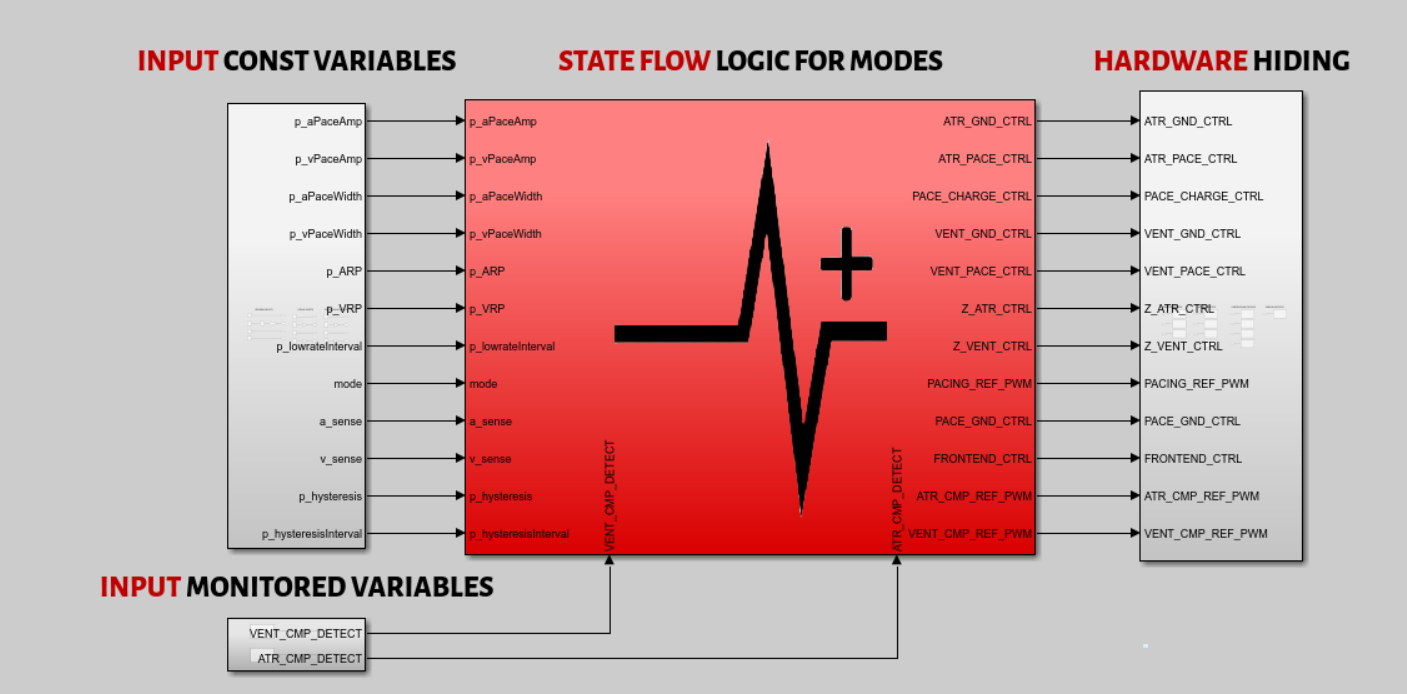
\includegraphics[width=\textwidth]{SimWholeView.png}
        \caption{Overall Simulink Mapping}
        \label{SimWholeView}
    \end{figure}
\end{tcolorbox}
The Pacemaker architecure can be split up into 4 main modules, input constant variables, 
input monitor variables, stateflow logic for modes, and hardware hiding. \hyperref[SimWholeView]{Figure 1} below shows the overarcing 
workflow of the system:

\newpage
\subsubsection{Input Constant Variables}

\begin{tcolorbox}
    \begin{figure}[H]
        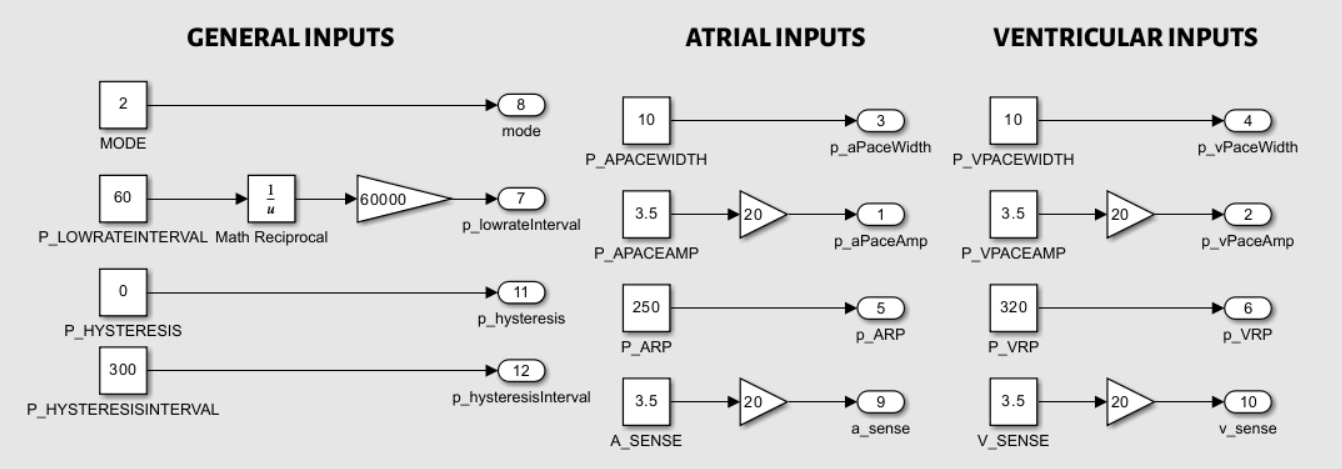
\includegraphics[width=\textwidth]{ConstIn.png}
        \caption{Constant Input Variables}
        \label{ConstIn}
    \end{figure}
\end{tcolorbox}
In the above image, \hyperref[ConstIn]{Figure 2}, we find changeable variables 
relating to pacemaker operation. For general inputs, the changeable variables are:

\begin{itemize}
    \item \textbf{Mode} - Refers to bradycardia operating modes, e.g AOO, VOO, AAI and VVI.
    \item \textbf{Low Rate Interval} - The number of generated pace pulses per minute.
    \item \textbf{Hysteresis Pace} - When enabled, a longer period is waited before pacing after sensing an event.
    \item Hysteresis Interval 
\end{itemize}
The modfiable atrial variables are:

\begin{itemize}
    \item \textbf{Pace Pulse Width} - Changes the width of the pace pulse
    \item \textbf{Pace Pulse Amplitude} - Changes the amplitude of the pace pulse
    \item \textbf{ARP (Atrial Refactory Period)} - The programmed time interval following an atrial event during which time atrial
            events shall not inhibit nor trigger pacing
    \item \textbf{Sense} - 
\end{itemize}
The modifiable ventricular variables are:

\begin{itemize}
    \item \textbf{Pace Pulse Width} - Changes the width of the pace pulse
    \item \textbf{Pace Pulse Amplitude} - Changes the amplitude of the pace pulse
    \item \textbf{VRP (Ventricle Refactory Period)} - The programmed time interval following an ventricle event during which time atrial
            events shall not inhibit nor trigger pacing
    \item Sense
\end{itemize}

\newpage
\subsubsection{Monitored Input Variables}

\begin{tcolorbox}
    \begin{figure}[H]
        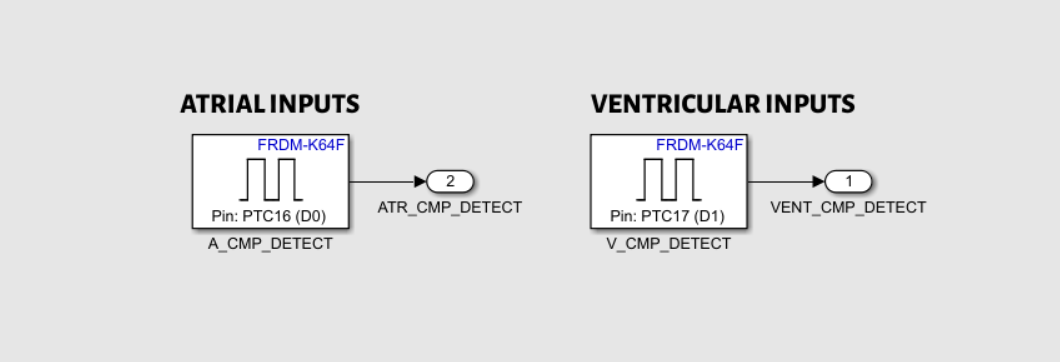
\includegraphics[width=\textwidth]{InMon.png}
        \caption{Monitored Input Variables}
        \label{InMon}
    \end{figure}
\end{tcolorbox}
The monitored input variables can be seen in the above \hyperref[InMon]{Figure 3}. These are the atrial and ventricle detection 
variables. The pulses are sensed with through GPIO pins connecting to a board simulating heart conditions. 

\newpage
\subsubsection{Stateflow Modules}
\begin{tcolorbox}
    \begin{figure}[H]
        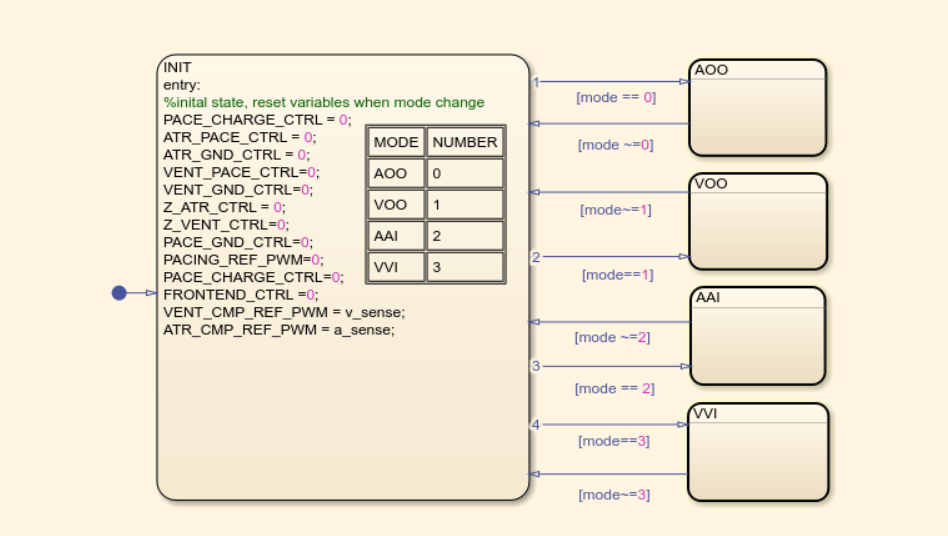
\includegraphics[width=\textwidth]{StateMod.png}
        \caption{Stateflow Modules}
        \label{StateMod}
    \end{figure}
\end{tcolorbox}
The stateflow diagram in Simulink is shown above. It shows the transition between each mode given the mode input shown in 
\hyperref[ConstIn]{Figure 2}. When switching between modes, a core state is returned to that resets variables to their nominal values. 

\newpage
\subsubsection{AOO Stateflow Model}
\begin{tcolorbox}
    \begin{figure}[H]
        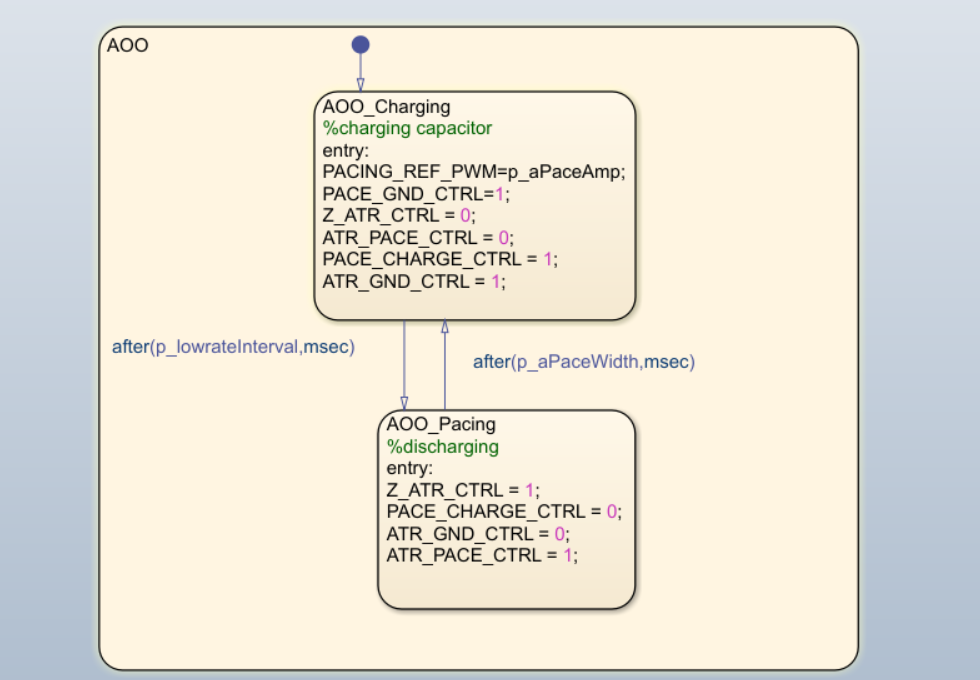
\includegraphics[width=\textwidth]{AOO.png}
        \caption{AOO Stateflow Model}
        \label{AOOSF}
    \end{figure}
\end{tcolorbox}
The above stateflow, \hyperref[AOOSF]{Figure 5}, shows the stateflow for the AOO mode. It sets values 
controlling discharge and charging of the capacitor to specified nominal values.

\newpage
\subsubsection{VOO Stateflow Model}
\begin{tcolorbox}
    \begin{figure}[H]
        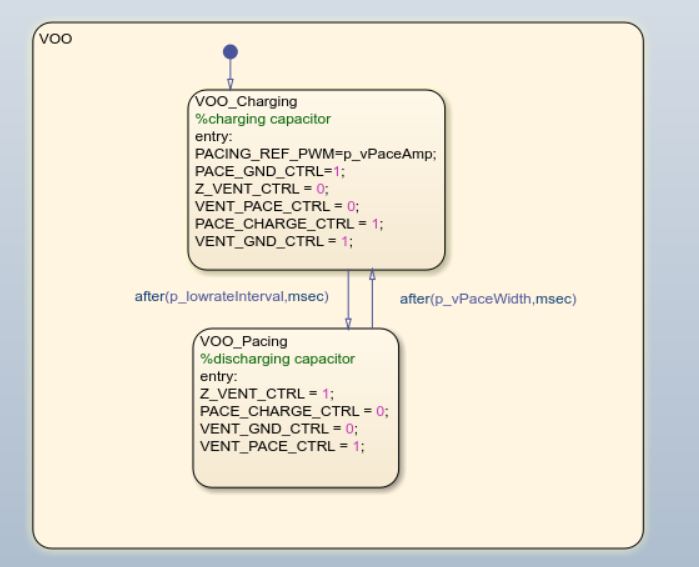
\includegraphics[width=\textwidth]{VOO.png}
        \caption{VOO Stateflow Model}
        \label{VOOSF}
    \end{figure}
\end{tcolorbox}
Similar to the AOO stateflow, the above figure, \hyperref[VOOSF]{Figure 6}, shows the states of 
charging and discharging of the capacitor using specified nominal values. 

\newpage
\subsubsection{VII Stateflow Model}
\begin{tcolorbox}
    \begin{figure}[H]
        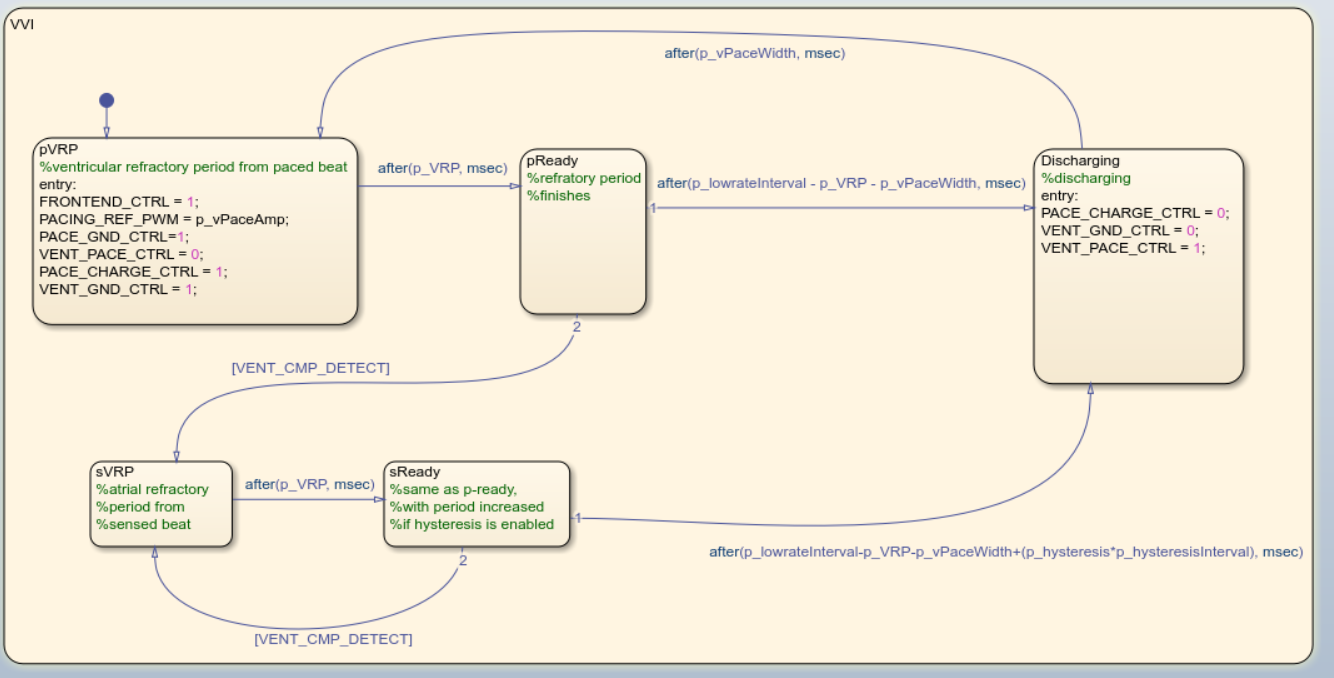
\includegraphics[width=\textwidth]{VVI.png}
        \caption{VVI Stateflow Model}
        \label{VVISF}
    \end{figure}
\end{tcolorbox}
The above stateflow, \hyperref[VVISF]{Figure 7} shows the FSM for the VVI model. The initial state, pVRP, is the state 
that occurs right after the pacemaker delivers a ventricle pacing pulse. A refactory period occurs during this time, where the 
pacemaker ignores sensor inputs to prevent sensing of its own produced pulse or electrical ringing. After a certain amount of time,
the pReady state is transitioned to where sensor inputs are allowed. This allows for the pacemaker to detect natural heart rhythms
and correct heart rhythms accordingly, or solely deliver pacing pulses. The last state before going to the initial state is the 
discharging state where the pacing pulse is produced. 

\newpage
\subsubsection{AAI Stateflow Model}
\begin{tcolorbox}
    \begin{figure}[H]
        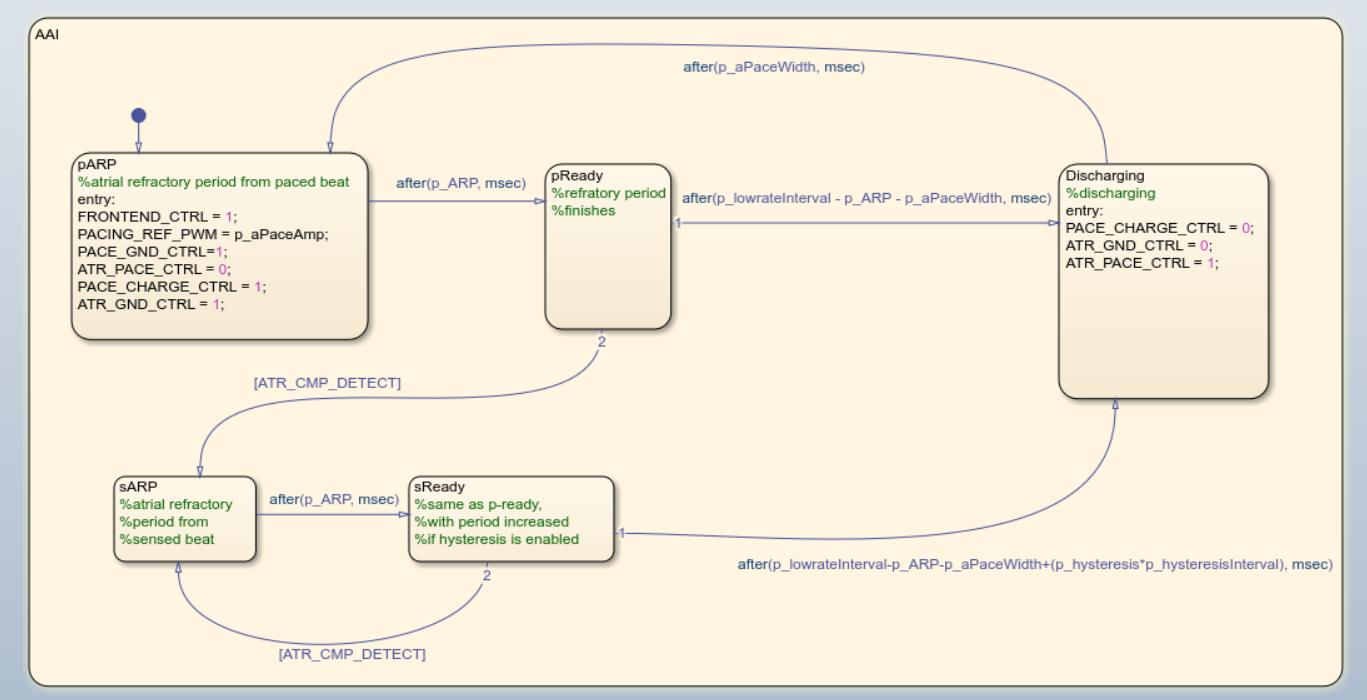
\includegraphics[width=\textwidth]{AAI.png}
        \caption{AAI Stateflow Model}
        \label{AAISF}
    \end{figure}
\end{tcolorbox}
The above stateflow, \hyperref[AAISF]{Figure 8} shows the process for the AAI mode. The initial state, pARP, is 
the state occurs right after the pacemaker delivers an atrial pacing pulse. During this time, the pacemaker ignores 
sensing events to prevent it from sensing its own delivered pulse. The next state is transitioned to after 
a set time period, the refactory period, if no natural heartbeat is detected after a certain time inverval, the 
discharging state is then transitioned to. However, if a natural heartbeat is detected, another refactory period occurs 
to prevent the pacemaker from sensing ringing. This state then transitions to the discharging state once an appropriate time 
has passed. 

\newpage
\subsubsection{Hardware Hiding}

\begin{tcolorbox}
    \begin{figure}[H]
        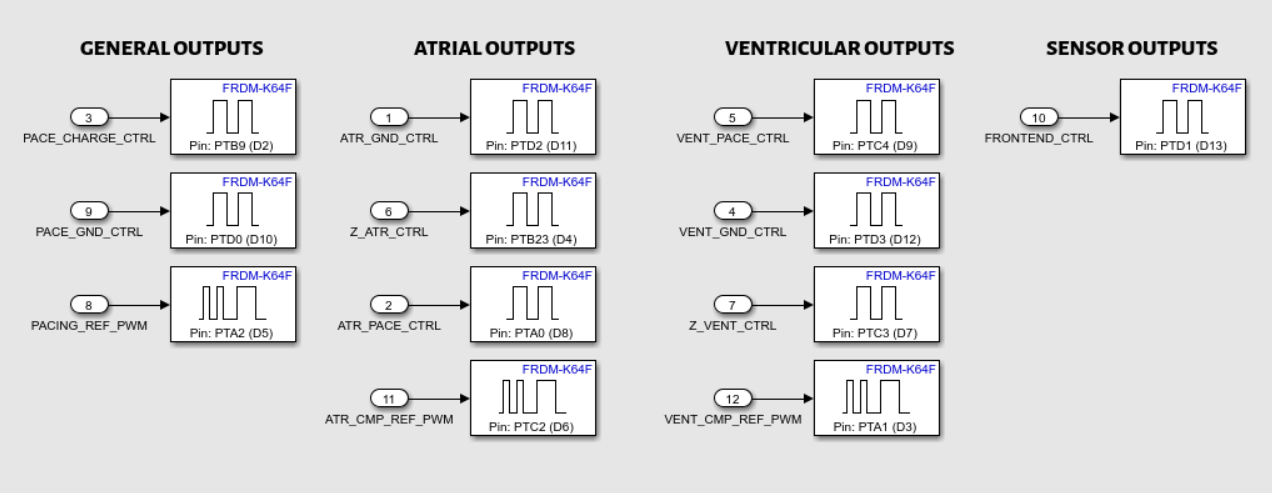
\includegraphics[width=\textwidth]{HardwareHiding.png}
        \caption{Hardware Hiding of Model}
        \label{HardHide}
    \end{figure}
\end{tcolorbox}

The above image, \hyperref[HardHide]{Figure 9} shows abstraction of the GPIO pin functions. 
It connects logical output signals to the pins on the FRDM-K64F. This allows for better readability,
thus making the code easier to maintain, debug and safer. 



\section{Part 2}

\subsection{Requirements Potential Changes}
Identify which requirements may evolve in the next deliverable (e.g., adding more modes, communication, new parameters).

\subsection{Design Decision Potential Changes}
List design choices that may need revisiting (e.g., choice of libraries, interface design, architecture).

\subsection{Module Description}
\begin{itemize}
    \item Purpose of the component
    \item Key functions/methods (public vs internal)
    \item Global or state variables (if any)
    \item Interactions with other components
\end{itemize}

\subsection{Testing}
Document test cases for each module. Each test case should include:

\begin{enumerate}
    \item Purpose of the test
    \item Input conditions
    \item Expected output
    \item Actual output
    \item Result (Pass/Fail)
\end{enumerate}

\begin{tcolorbox}
    \begin{figure}[H]
        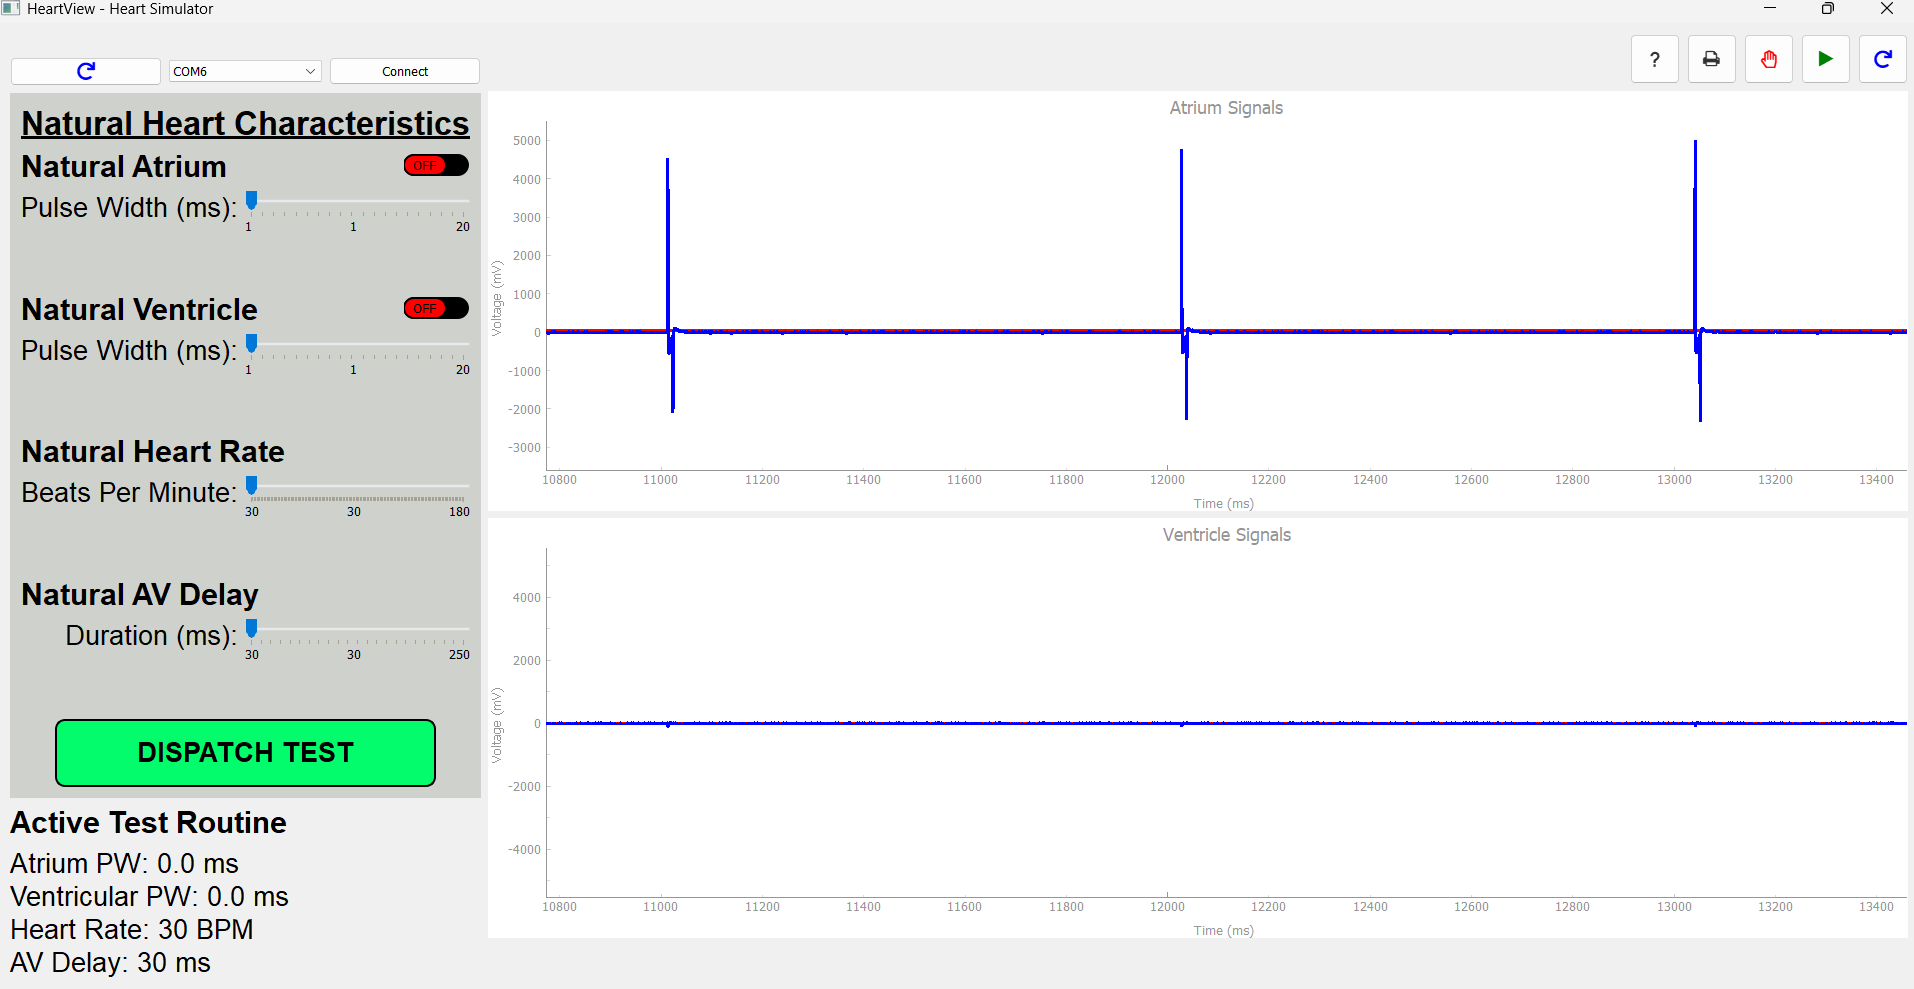
\includegraphics[width=\textwidth]{AOOtest1.png}
        \caption{AOO Test}
        \label{AOOtest}
    \end{figure}
\end{tcolorbox}

\begin{tcolorbox}
    \begin{figure}[H]
        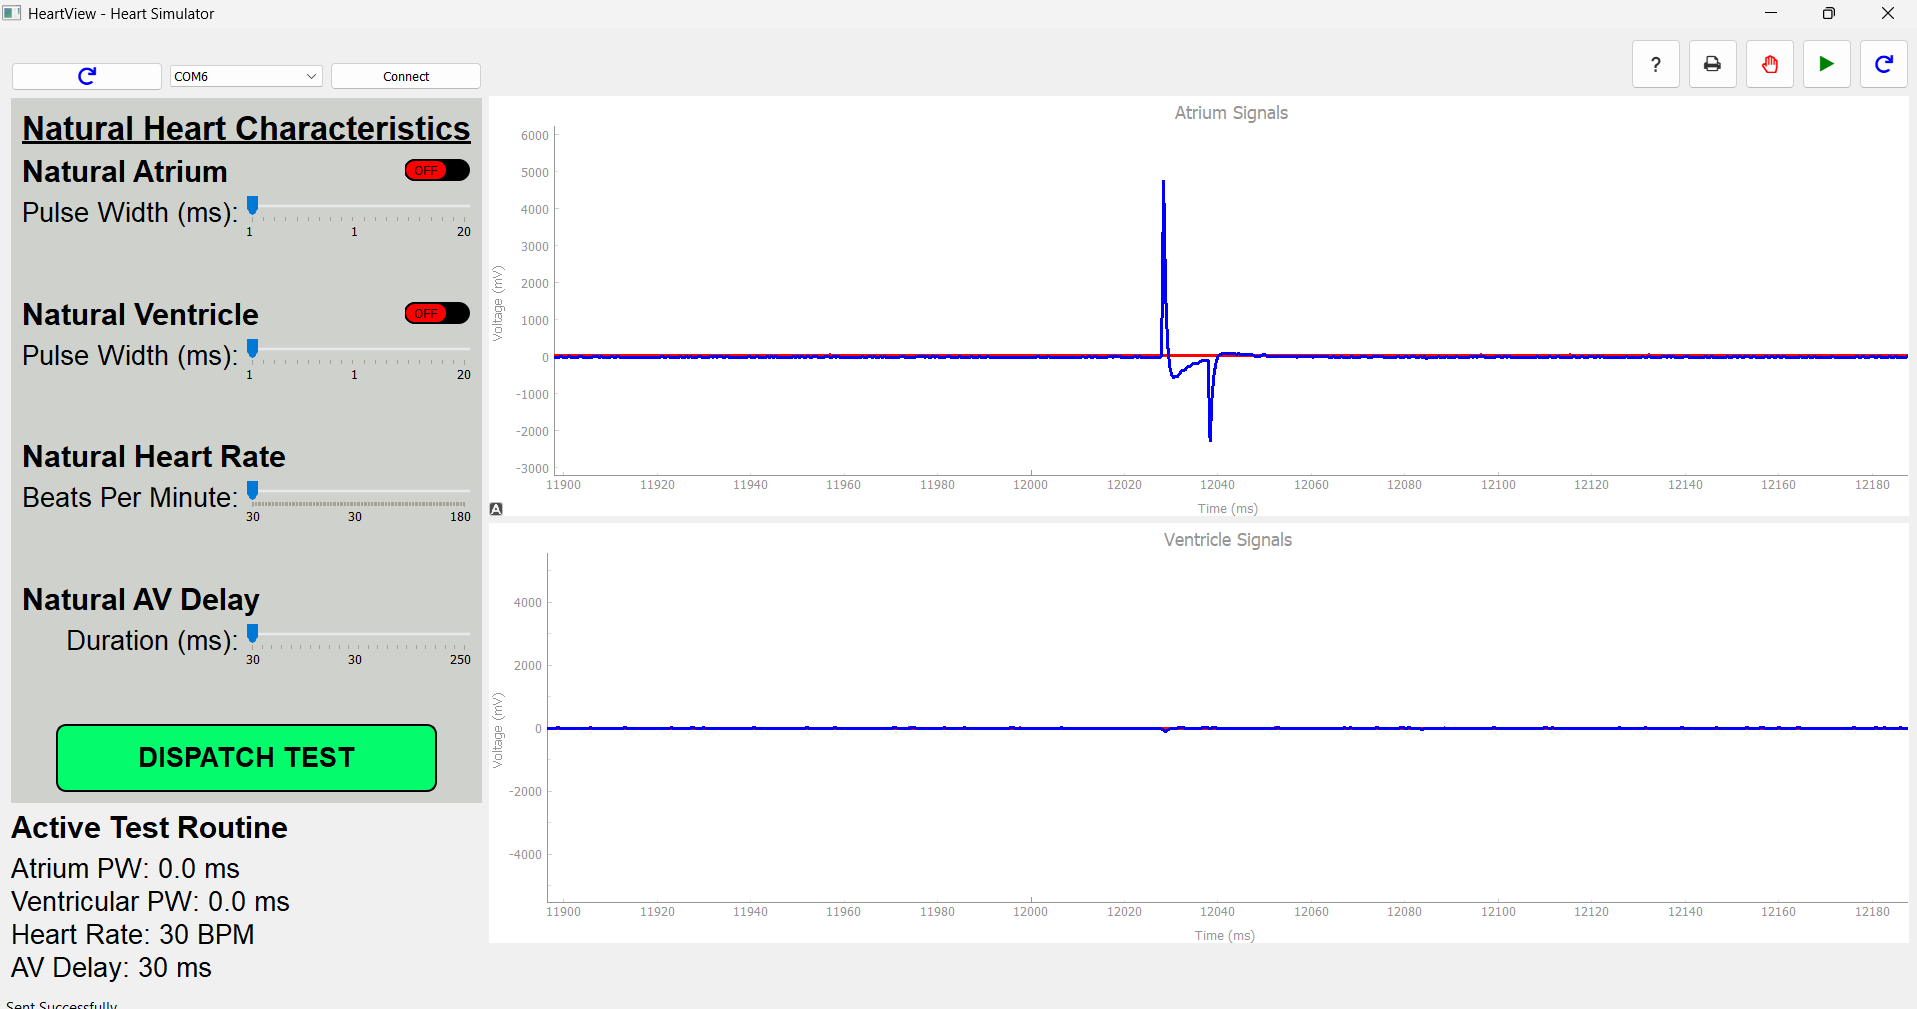
\includegraphics[width=\textwidth]{AOOPulseClose.png}
        \caption{Close-up of AOO Pulse}
        \label{AOOpulse}
    \end{figure}
\end{tcolorbox}

\begin{tcolorbox}
    \begin{figure}[H]
        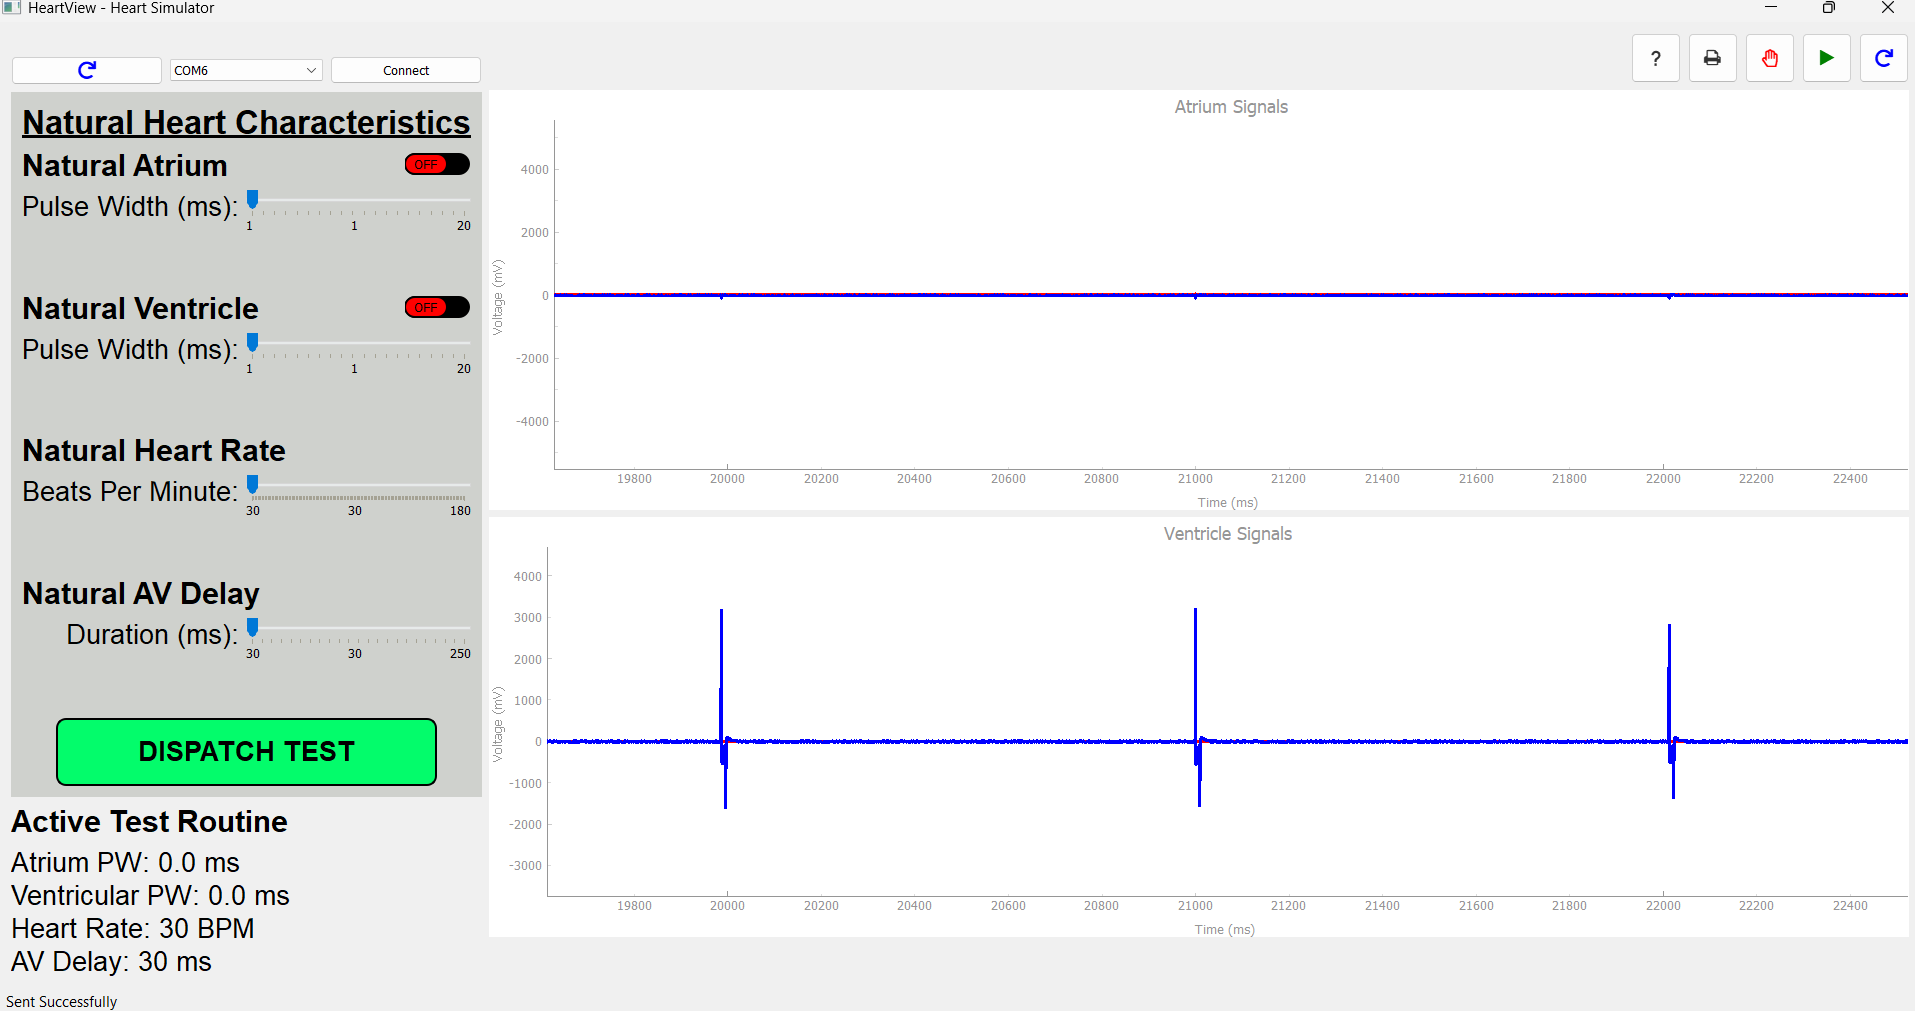
\includegraphics[width=\textwidth]{VOOtest.png}
        \caption{VOO Test}
        \label{VOOpulse}
    \end{figure}
\end{tcolorbox}

\begin{tcolorbox}
    \begin{figure}[H]
        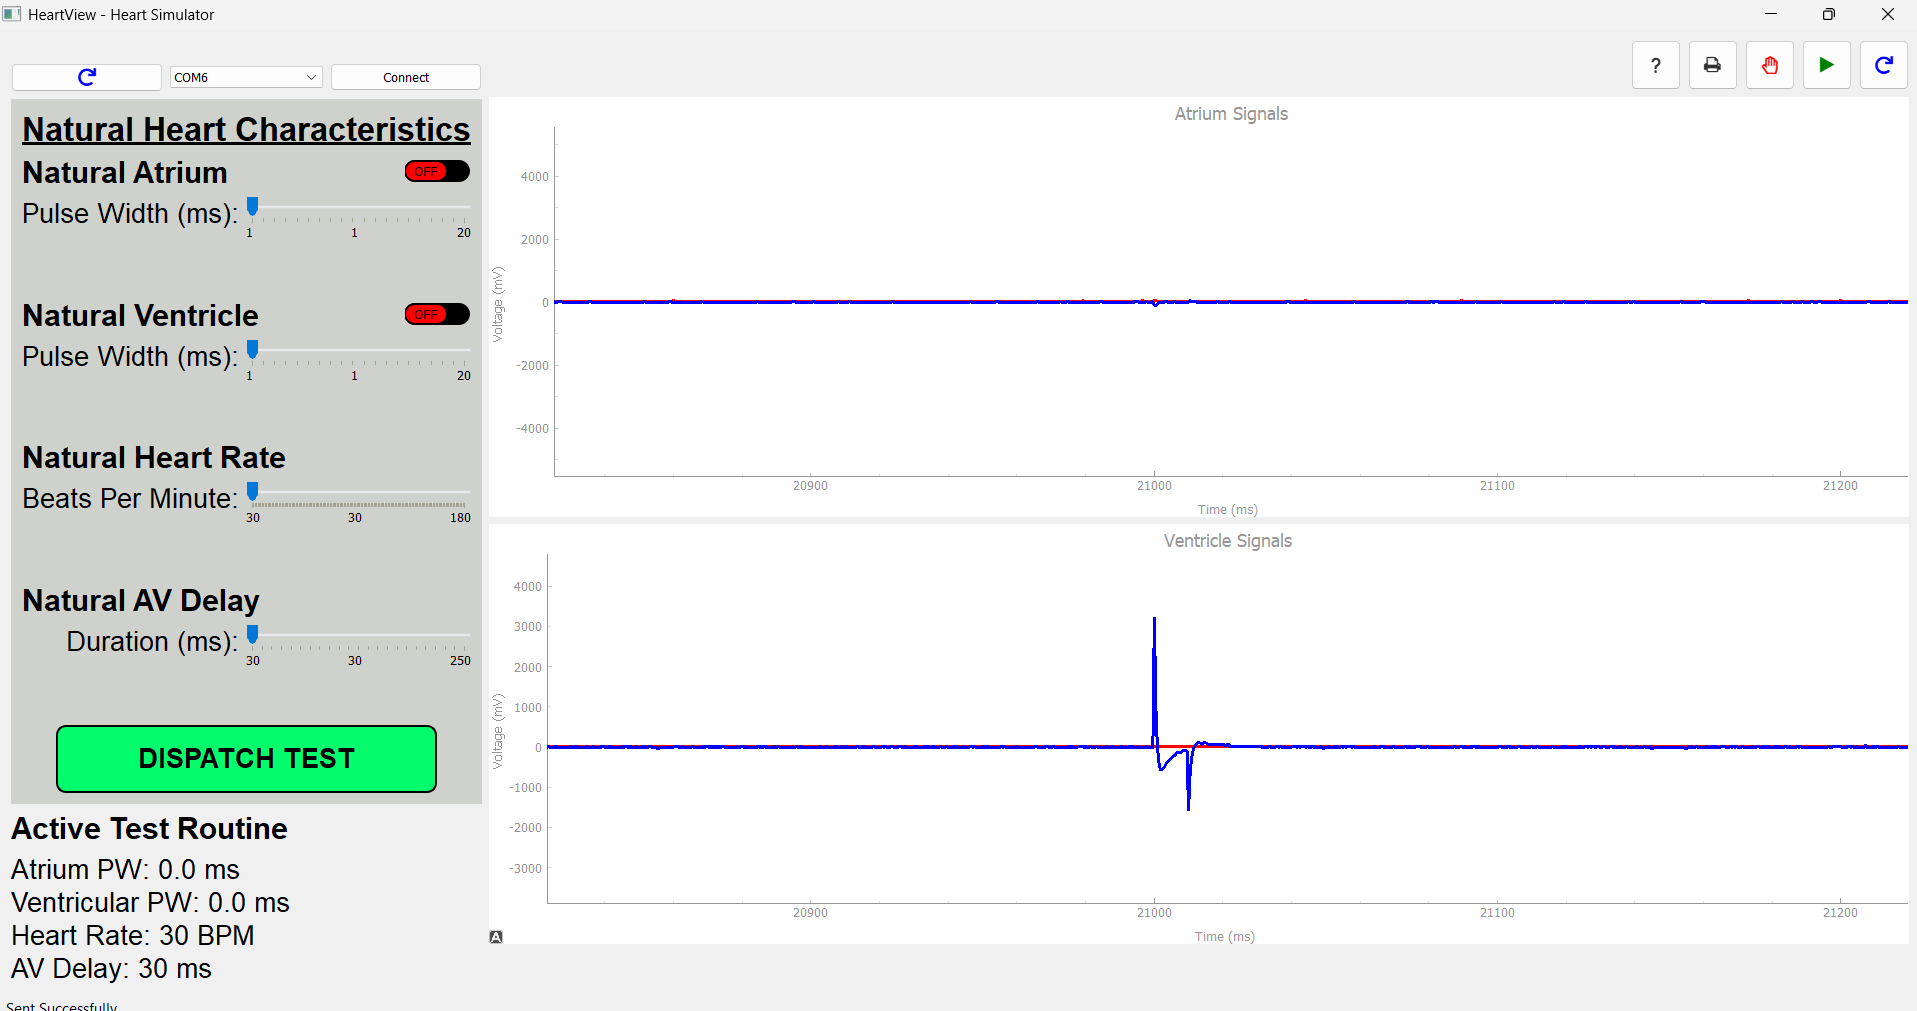
\includegraphics[width=\textwidth]{VOOpulseclose.png}
        \caption{Close-up of VOO Pulse}
        \label{VOOpulse}
    \end{figure}
\end{tcolorbox}

\begin{tcolorbox}
    \begin{figure}[H]
        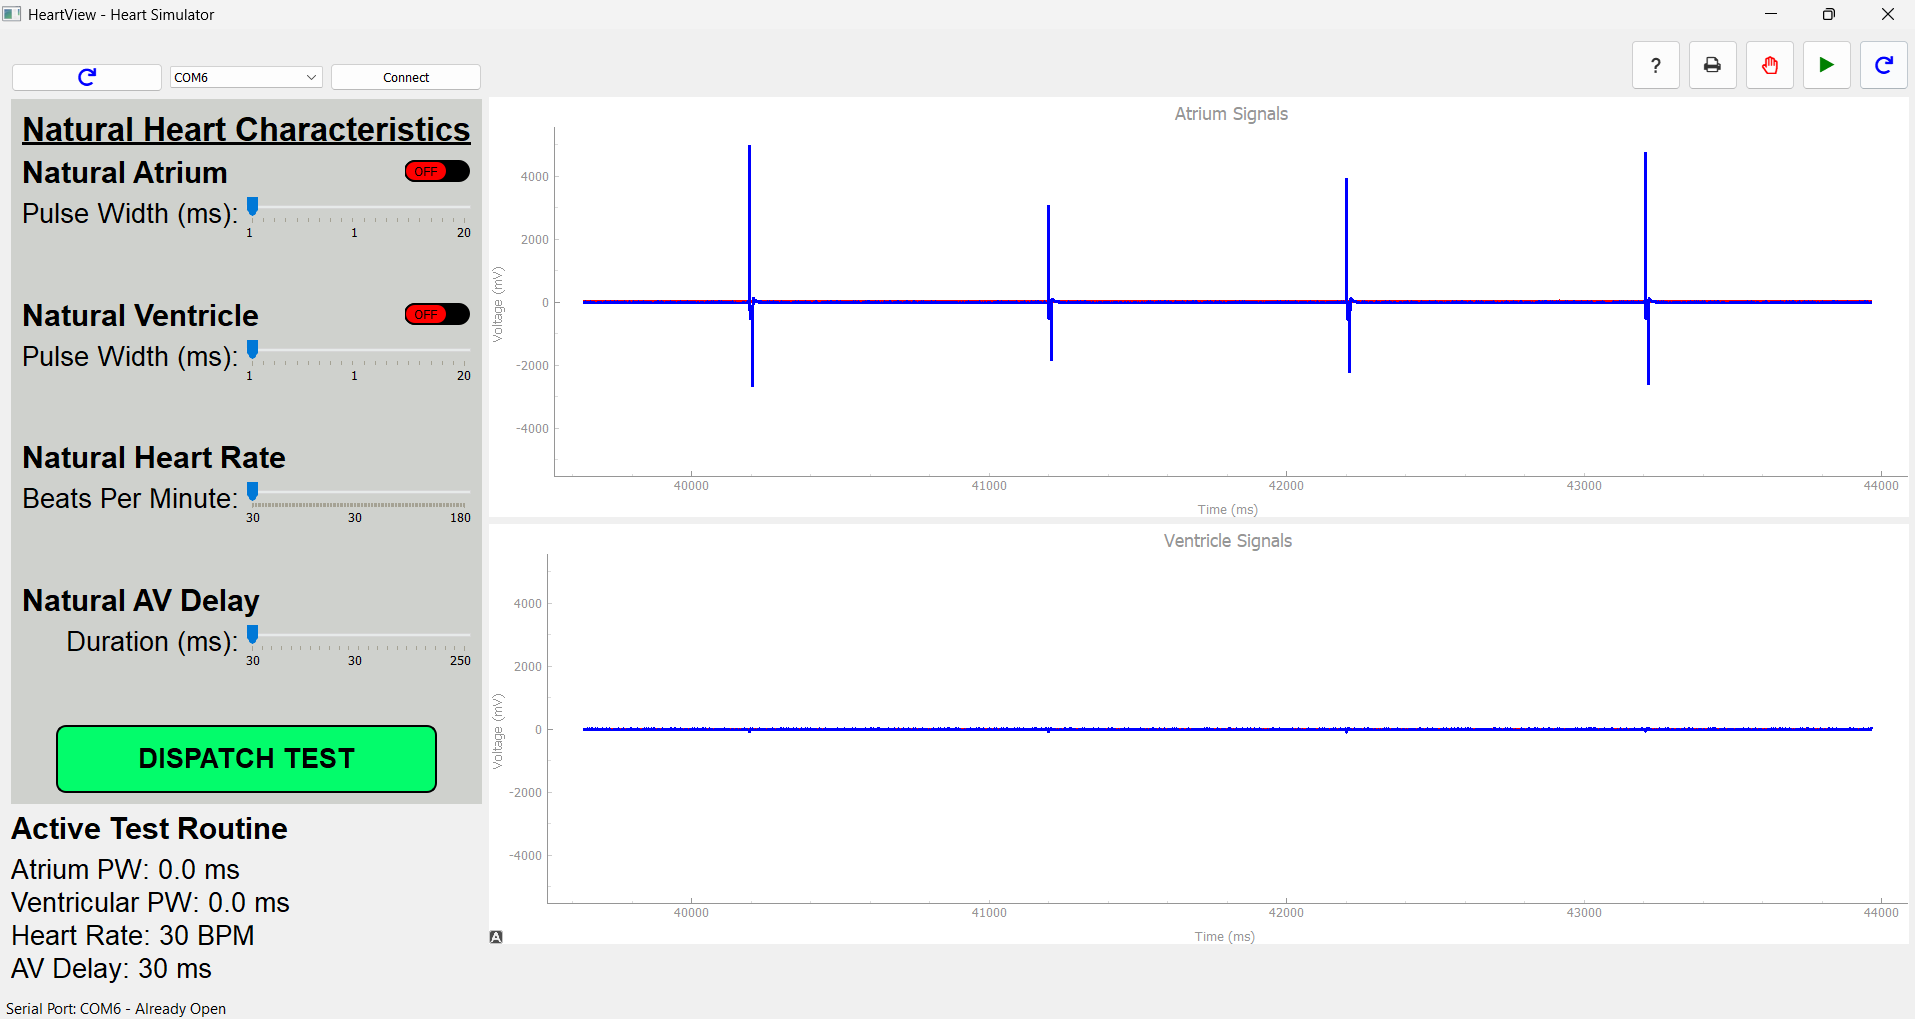
\includegraphics[width=\textwidth]{AAItestnohr.png}
        \caption{AAI Test No Heart Rate}
        \label{AAItestnohr}
    \end{figure}
\end{tcolorbox}

\begin{tcolorbox}
    \begin{figure}[H]
        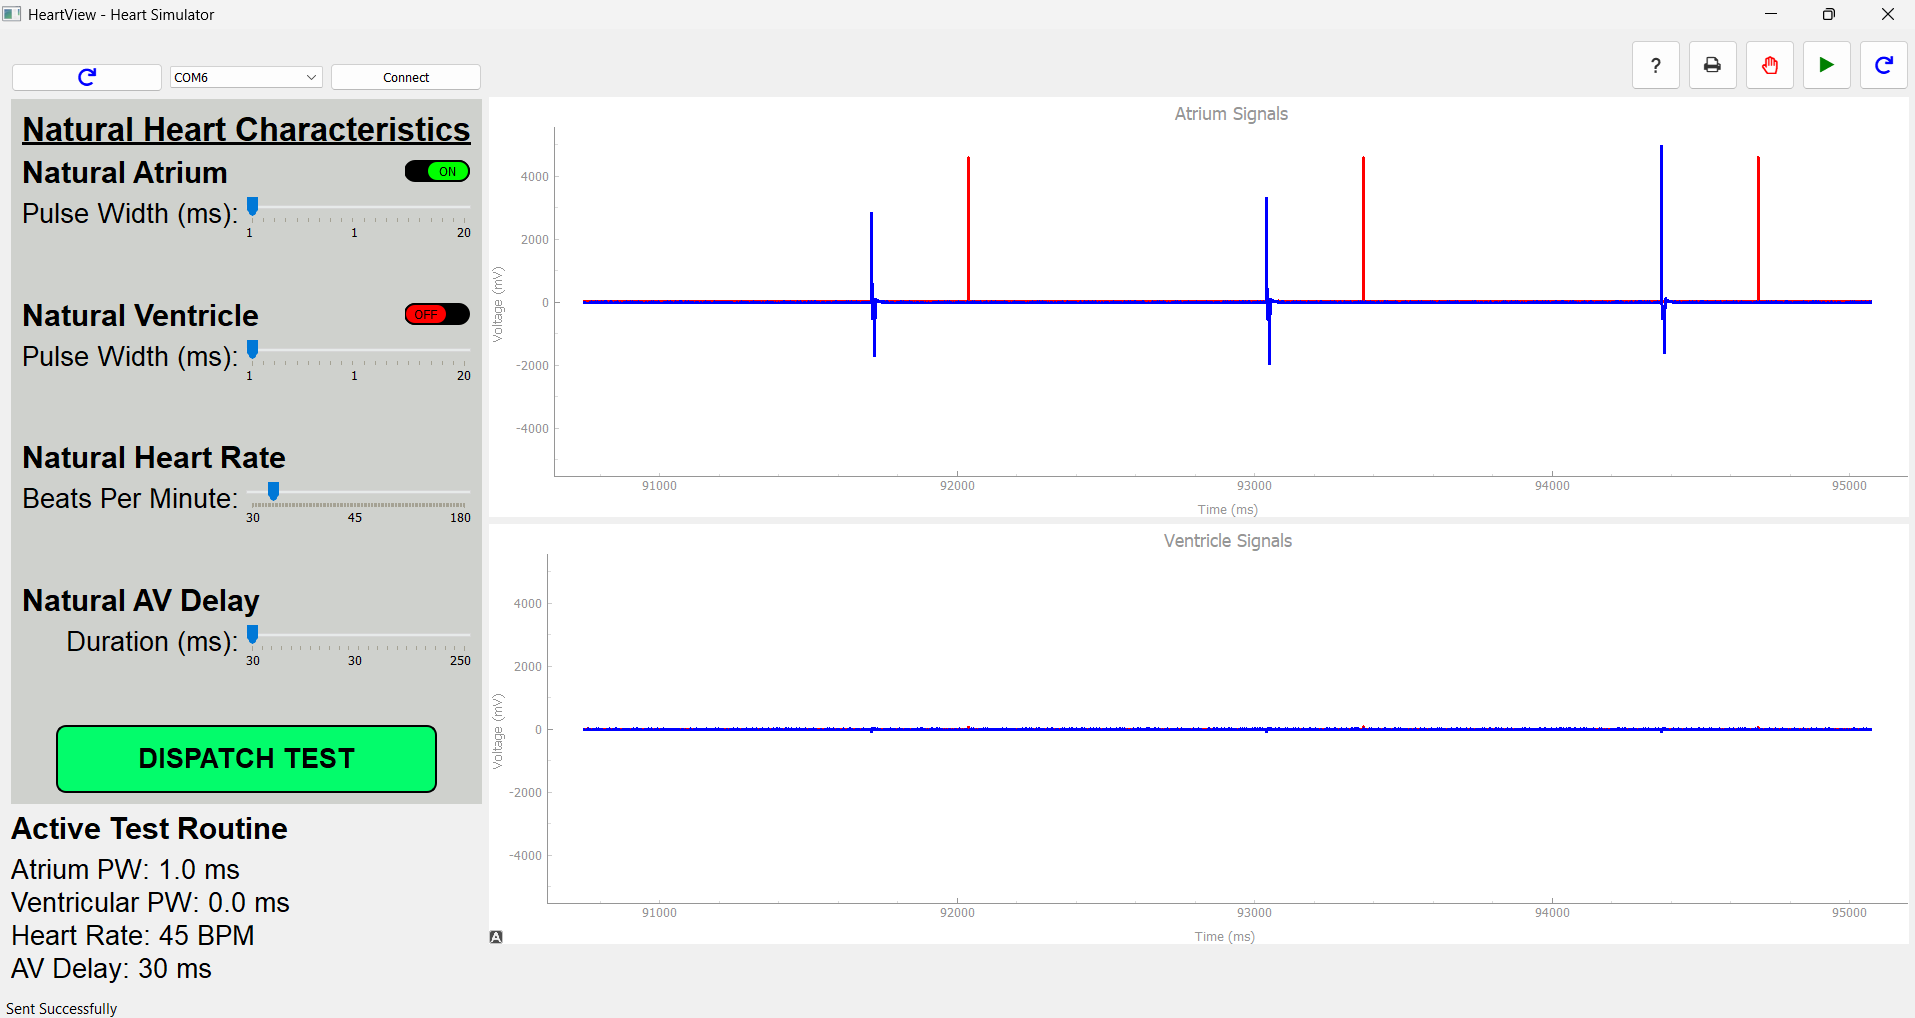
\includegraphics[width=\textwidth]{AAItest45.png}
        \caption{AAI Test 45 BPM}
        \label{AAItest45}
    \end{figure}
\end{tcolorbox}

\begin{tcolorbox}
    \begin{figure}[H]
        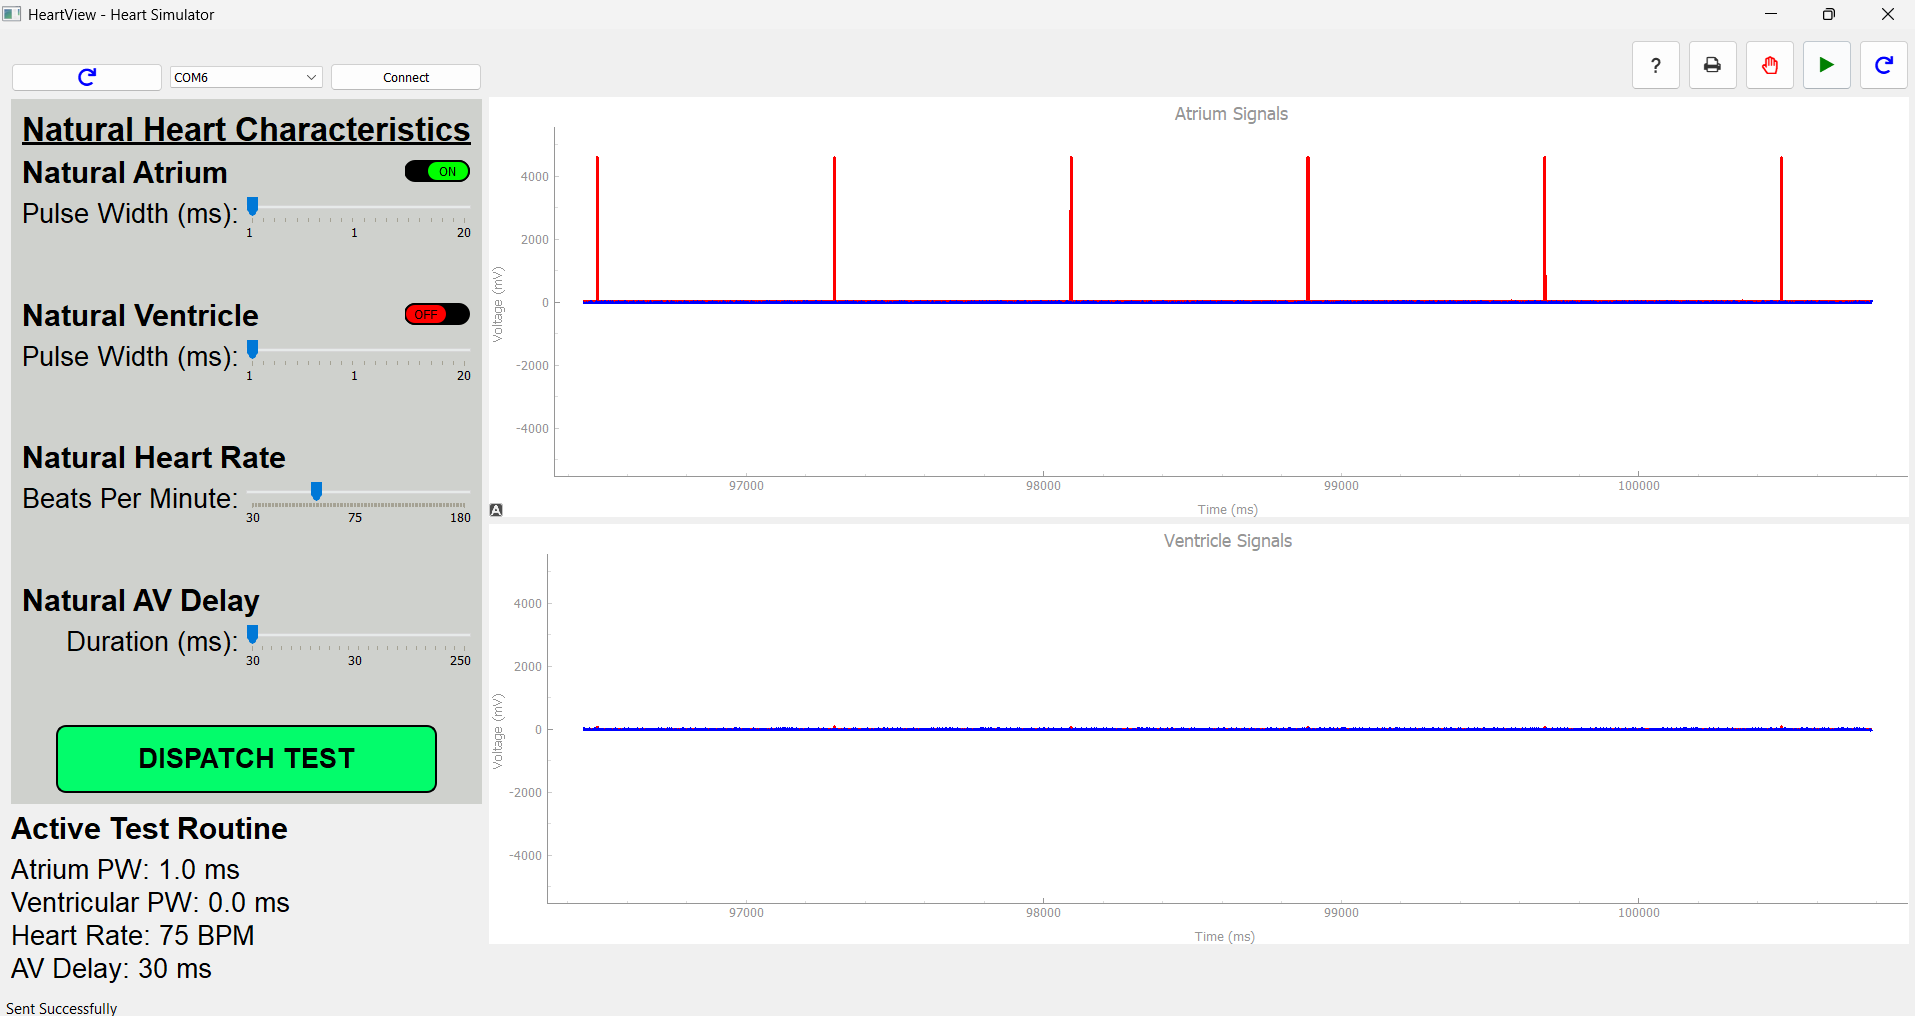
\includegraphics[width=\textwidth]{AAItest75.png}
        \caption{AAI Test 75 BPM}
        \label{AAItest75}
    \end{figure}
\end{tcolorbox}

\begin{tcolorbox}
    \begin{figure}[H]
        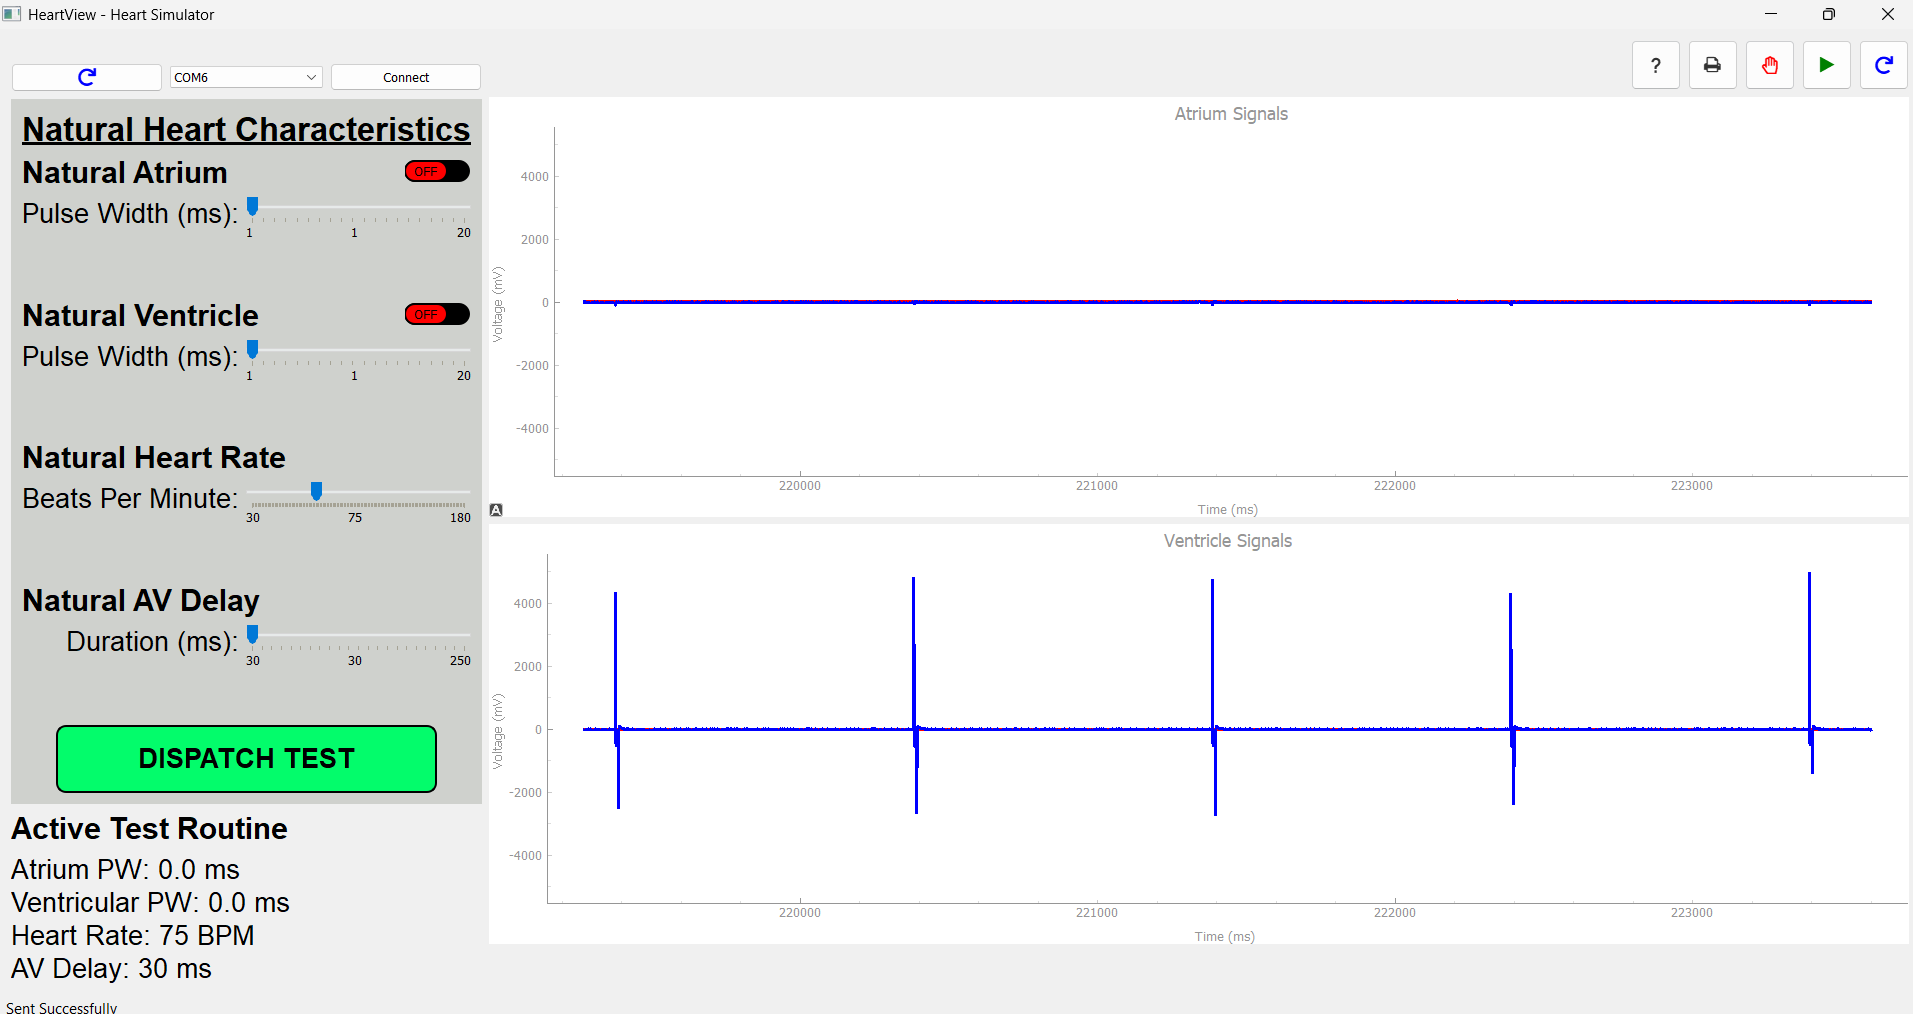
\includegraphics[width=\textwidth]{VVItestnohr.png}
        \caption{VVI Test No Heart Rate}
        \label{VVItestnor}
    \end{figure}
\end{tcolorbox}

\begin{tcolorbox}
    \begin{figure}[H]
        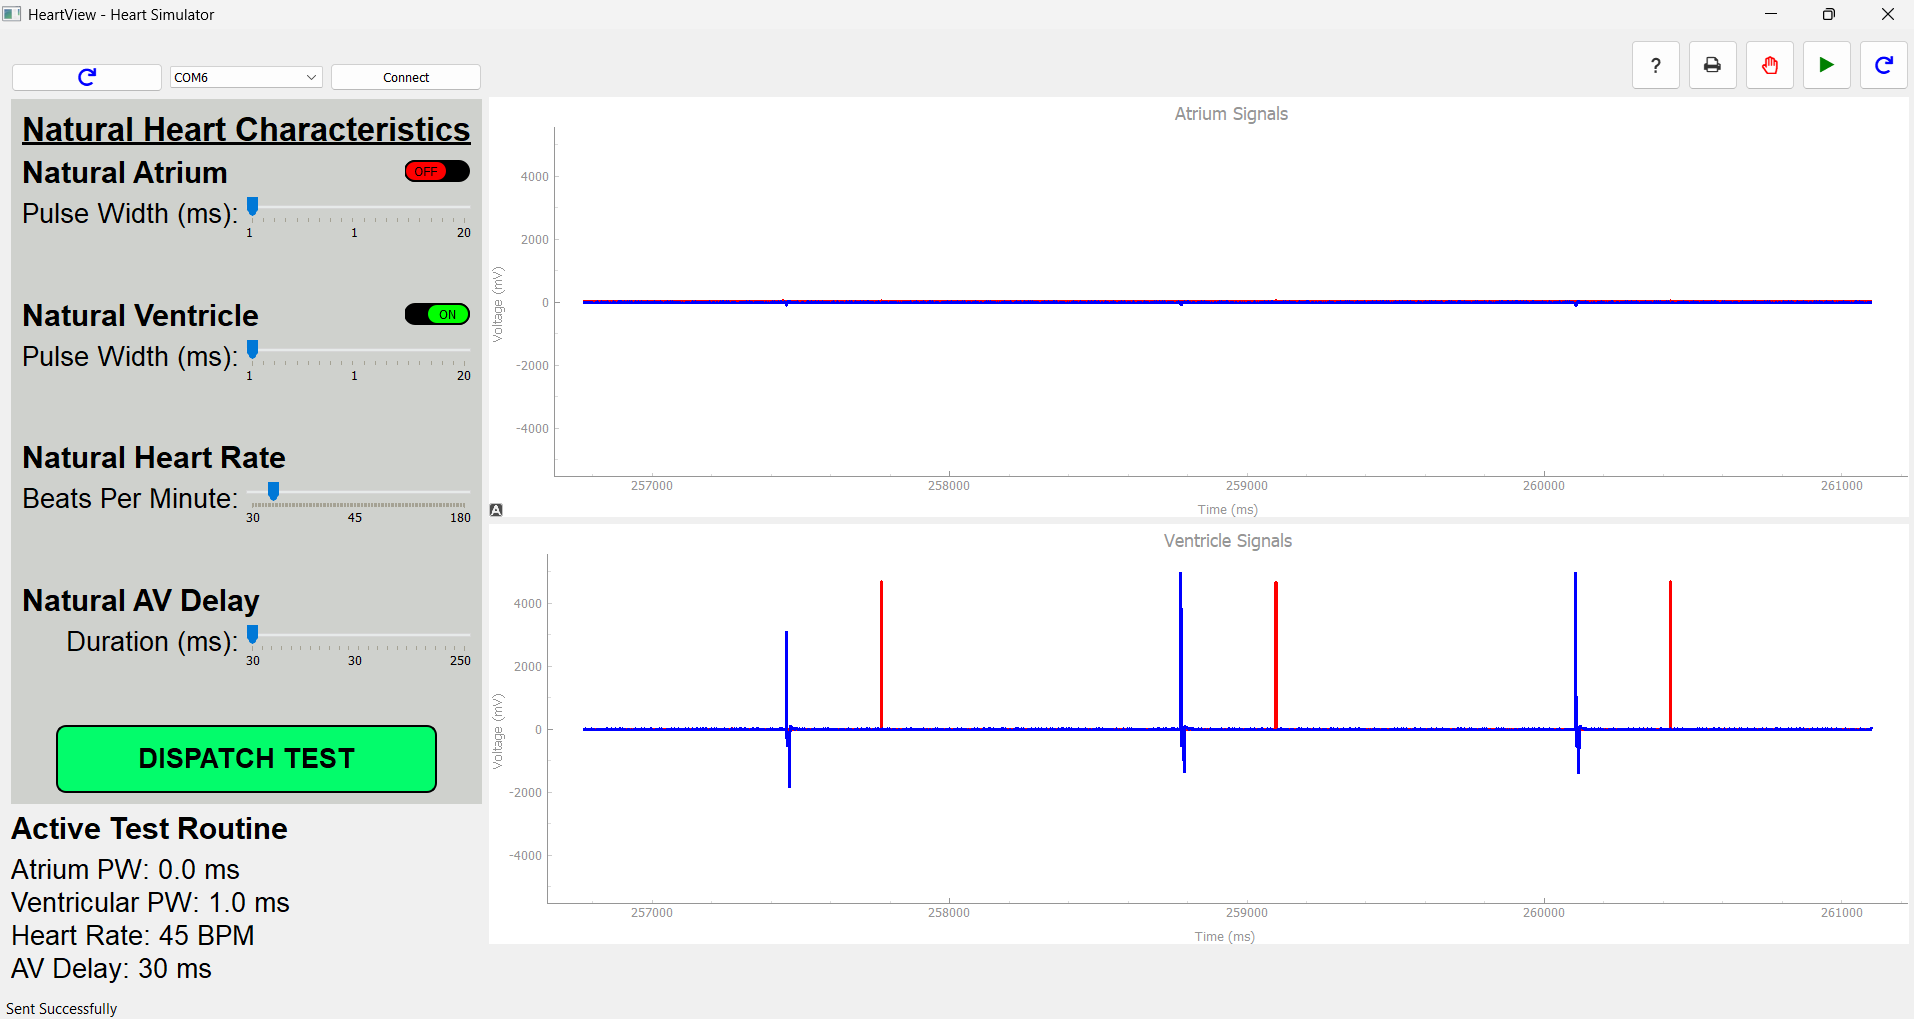
\includegraphics[width=\textwidth]{VVItest35.png}
        \caption{VVI Test 45 BPM}
        \label{VVItest45}
    \end{figure}
\end{tcolorbox}

\begin{tcolorbox}
    \begin{figure}[H]
        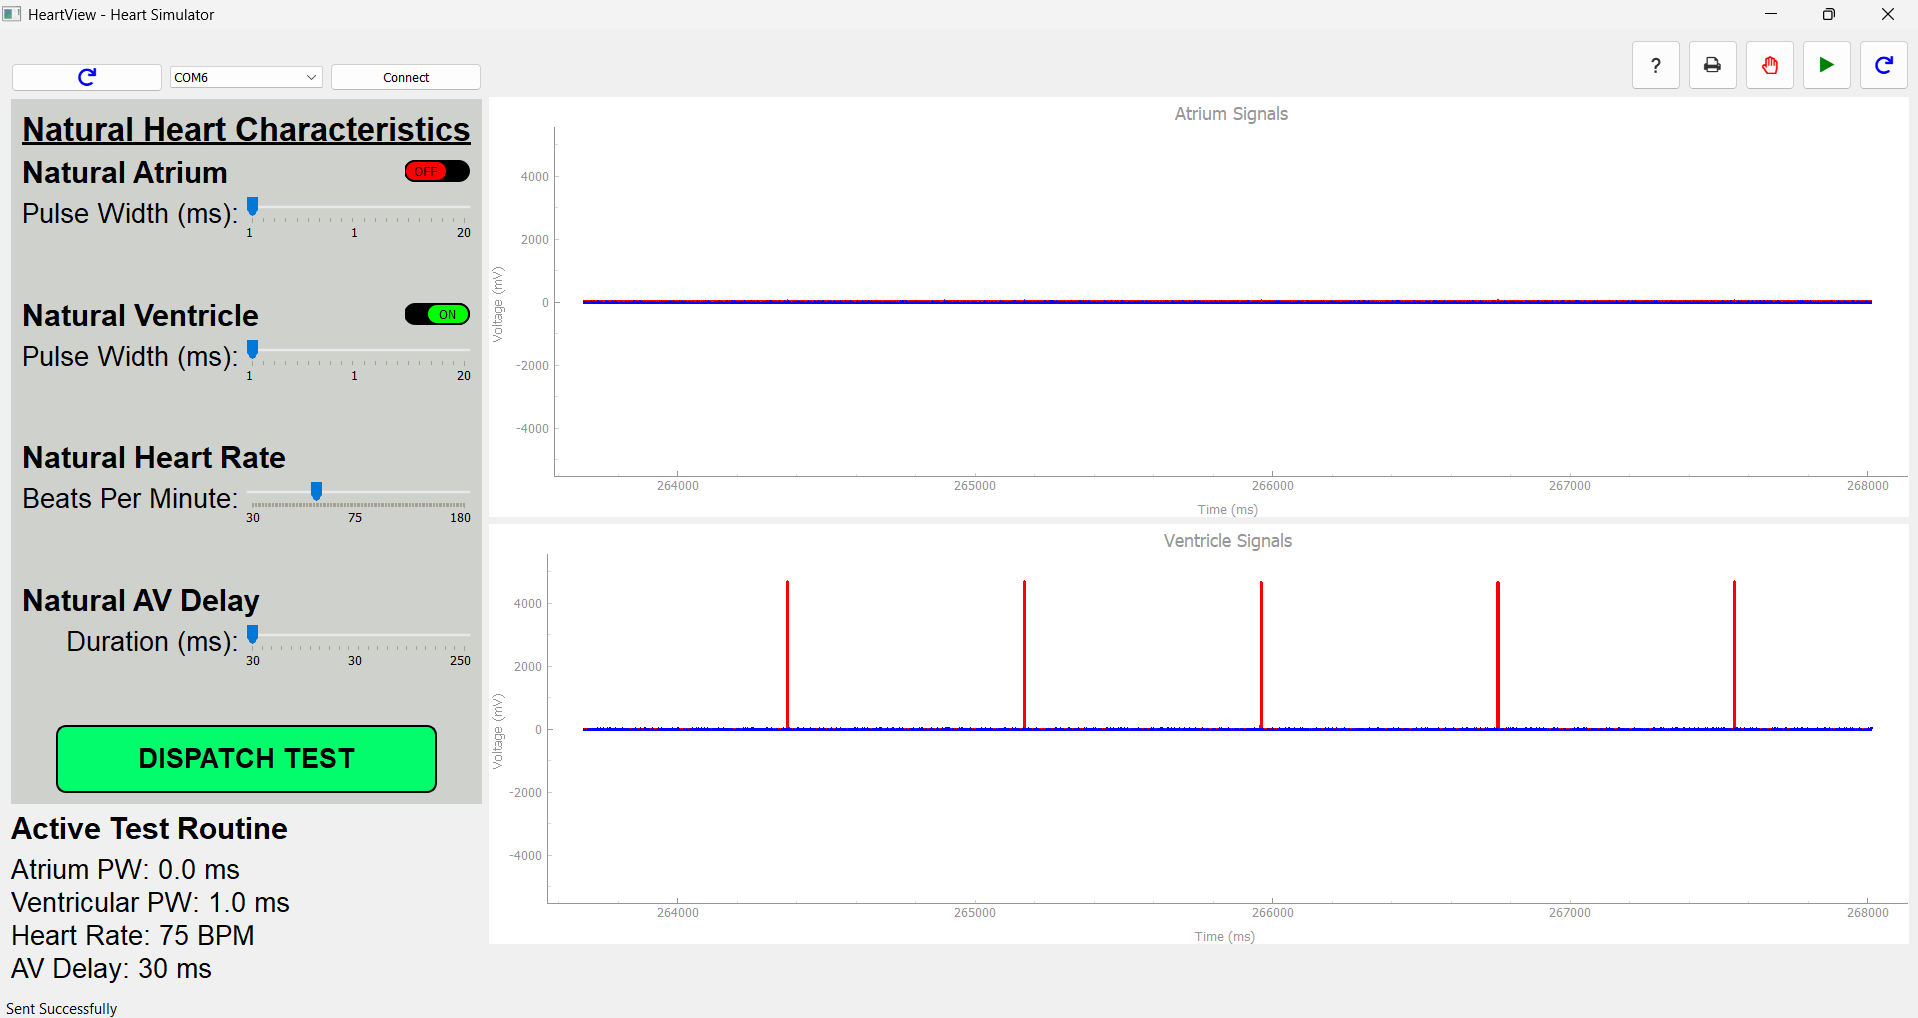
\includegraphics[width=\textwidth]{VVItest75.png}
        \caption{VVI Test 75 BPM}
        \label{VVItest75}
    \end{figure}
\end{tcolorbox}

\begin{tcolorbox}
    \begin{figure}[H]
        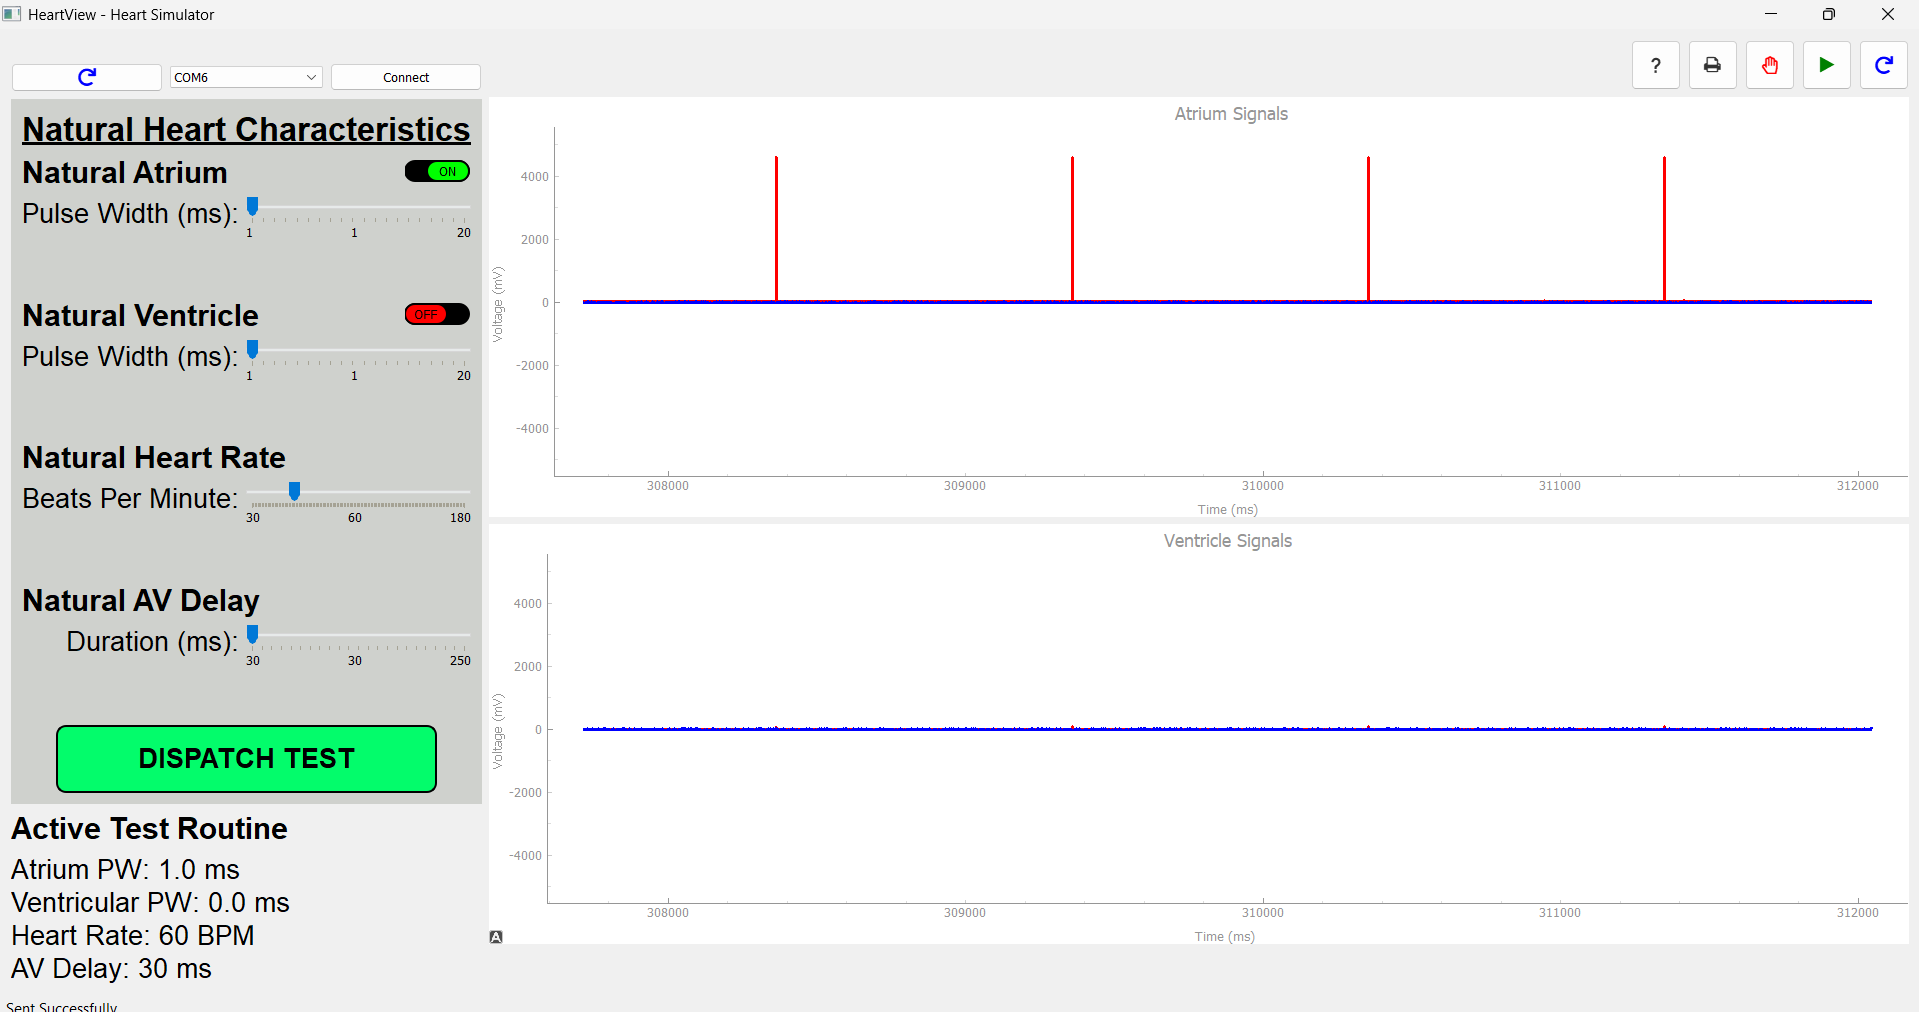
\includegraphics[width=\textwidth]{hystherisistest.png}
        \caption{Hysterisis Test 2}
        \label{Hystest1}
    \end{figure}
\end{tcolorbox}

\begin{tcolorbox}
    \begin{figure}[H]
        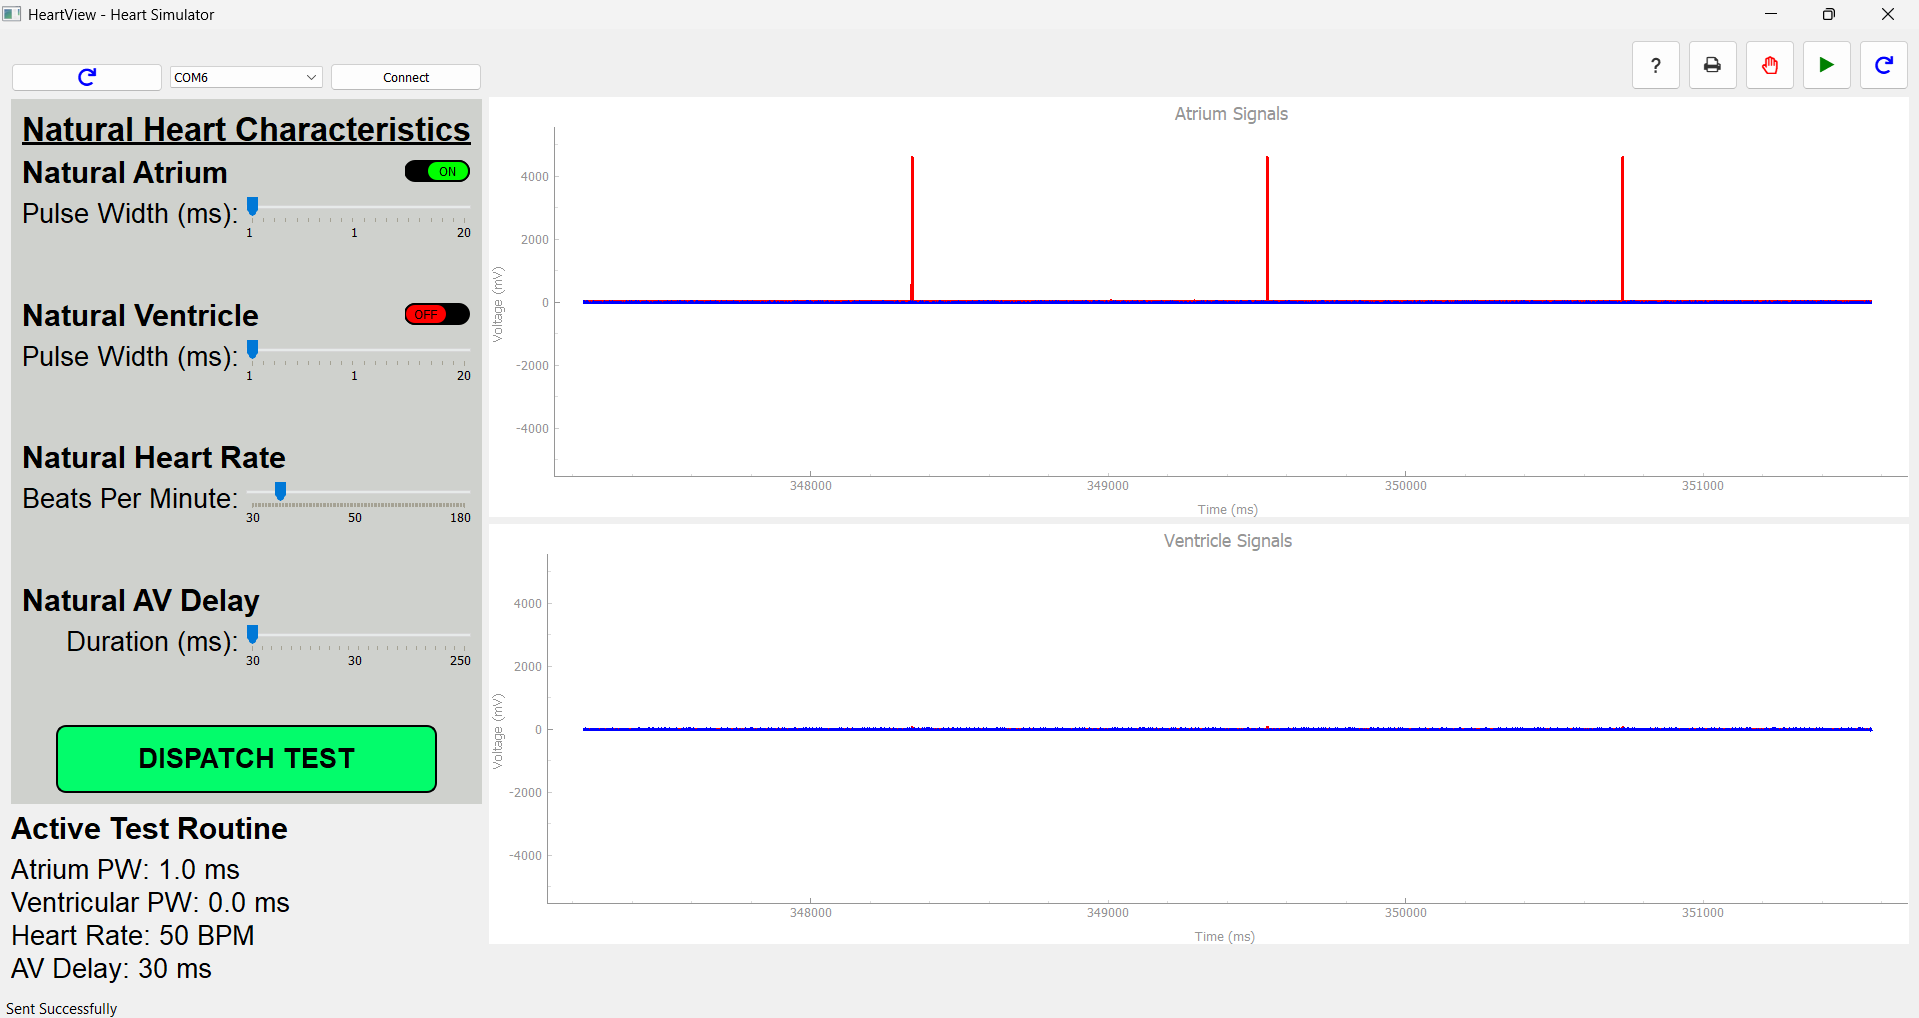
\includegraphics[width=\textwidth]{hythersistest2.png}
        \caption{Hysterisis Test 2}
        \label{Hystest2}
    \end{figure}
\end{tcolorbox}

\begin{tcolorbox}
    \begin{figure}[H]
        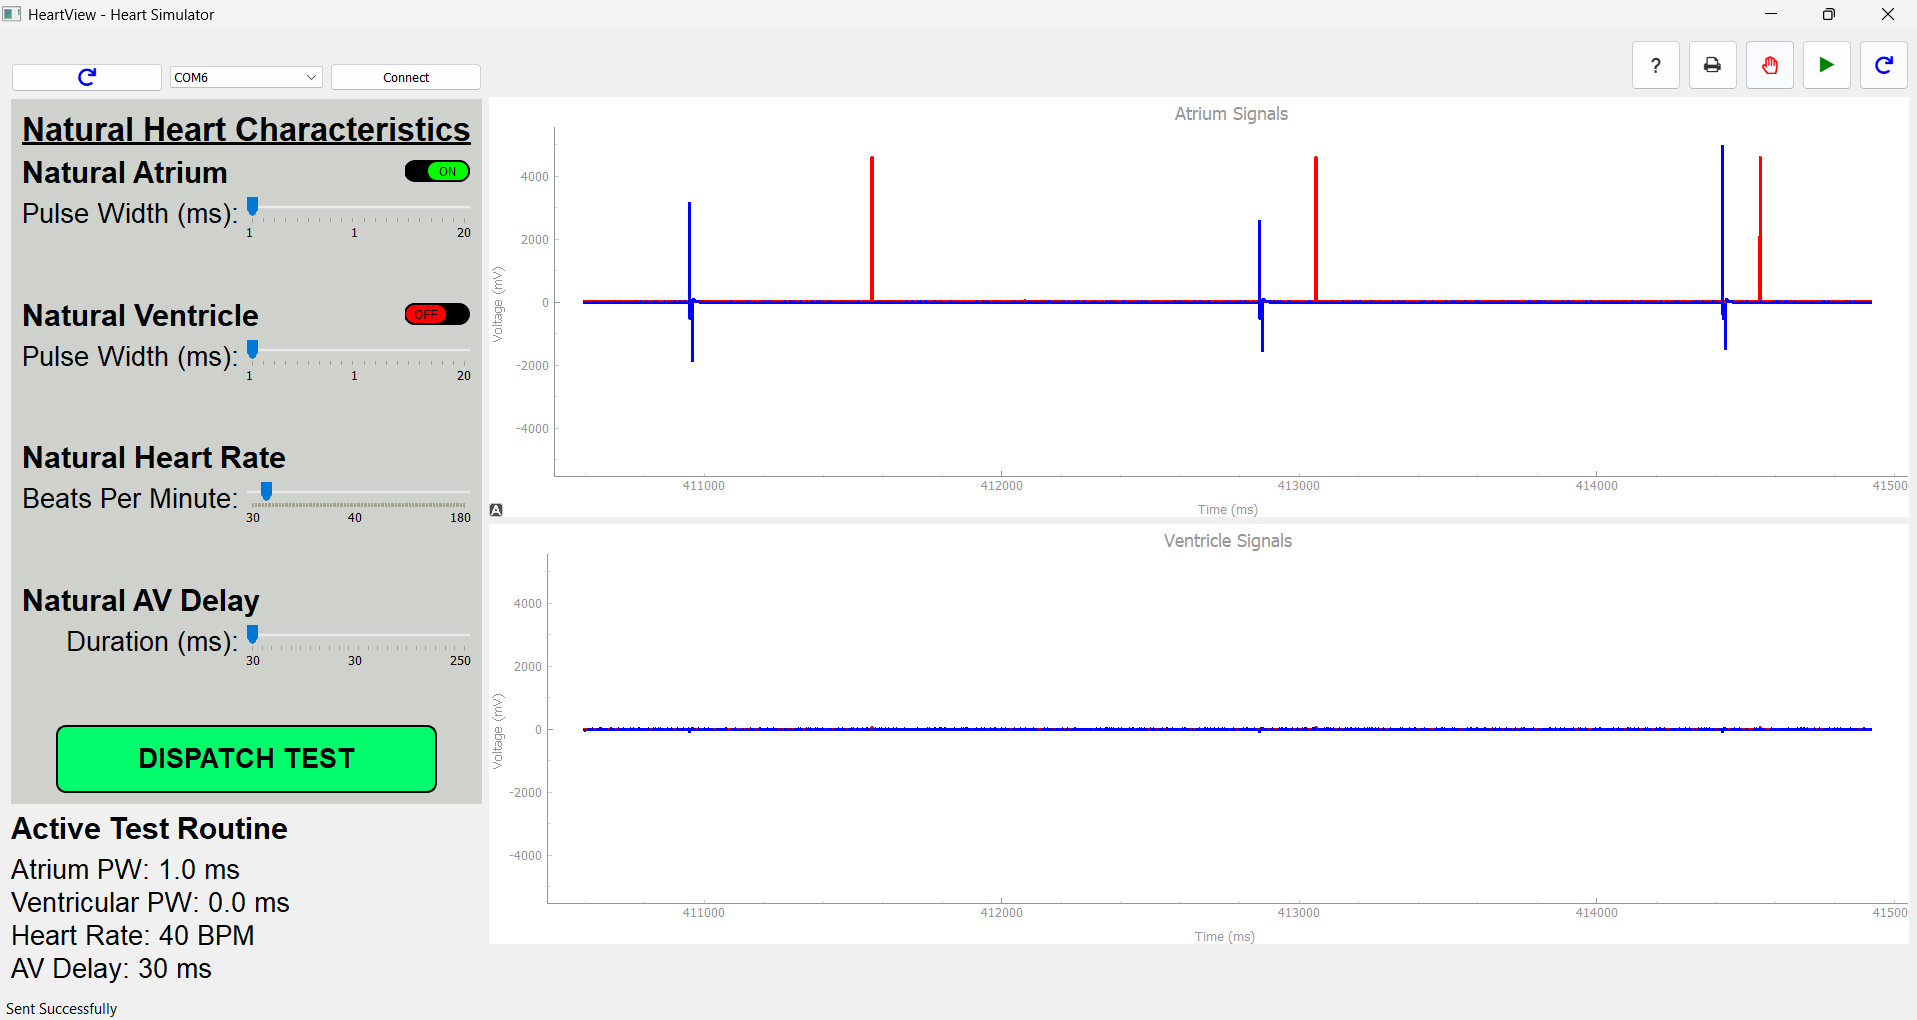
\includegraphics[width=\textwidth]{hytheresistest3.png}
        \caption{Hysterisis Test 3}
        \label{Hystest3}
    \end{figure}
\end{tcolorbox}

For instance, on the DCM side, you should test registration and login, parameter input validation, and mode selection and data storage/retrieval. This is not a complete list, depending on your system, you will need to test other components.

\subsection{GenAI Usage}
Provide a summary of any usage of GenAI in developing the model, DCM or writing this section. If you did not use GenAI tools at all, state that.

% ----------------------------------------------------
\section{General Notes}
\begin{itemize}
    \item This is a general outline based on the Deliverable 1 handout. You should make sure everything listed in the handout it is included. 
    \item Use screenshots of Simulink diagrams and DCM interface where appropriate.
    \item Ensure the requirements are traceable to design and test cases.
    \item Be concise and make things clear.
    \item You can add other sections, and you can also decide not to use this structure, however, I am including the main general sections we will expect to see.
\end{itemize}

\end{document}
